\chapter{The LUX-ZEPLIN Experiment}
\label{chap:chap2}

The introduction of dual-phase liquid xenon time-projection chambers, the origins of which date back to the 1970s, paved the way for substantial progress in the exploration of WIMP dark matter. The effective use of this technology made the LUX experiment the first sub-zeptobarn detector, placing stronger constraints on WIMP dark matter than all its predecessors. The next generation LUX-ZEPLIN (LZ) dark matter experiment, located in the Davis Cavern of the Sanford Underground Research Facility (Lead, South Dakota), 4850 feet under the ground, aims to build on this success in reaching ever-so sensitive WIMP-nucleon cross-sections. This section will introduce the concept of using xenon TPCs for direct detection dark matter searches; detailing the particle interactions, the detection mechanisms and providing an overview of the LZ detector.


%%------------------------------$$
%%------------------------------$$
\section{Dual-Phase Xenon TPCs}
\label{sec:dualphaseTPC}

The introduction of dual-phase TPC technology into the domain of direct detection over the past decade has dramatically improved the pace at which the sensitivity to WIMP dark matter has progressed. Dating back to the 1970s \cite{tpc_technology}, TPC technology has made possible the use of liquid and gaseous xenon as a scintillation media to detect particle interactions, leading to ever-more stringent limits on SI and SD WIMP-nucleon cross-sections across a wide range of WIMP masses. The two main variables that strongly impact the sensitivity to WIMPs are the background rates as observed in the WIMP region of interest (ROI) and the amount of xenon held within the TPC.

In comparison to other noble elements, xenon offers several advantages. The large atomic number of xenon, $A=131$, allows for a high sensitivity to SI-WIMP interactions due to the coherent scattering enhancement, $\propto A^2$, as given by equation \ref{eq:si_rate}. At relatively low energy thresholds (e.g. $\sim17$ keV for 100 GeV/c$^2$ WIMPs), xenon is the most sensitive noble element of these targets. A comparison of the SI differential event rate for a collection of targets is shown in figure \ref{fig:nuclear_recoil_rates}. The large atomic number also gives xenon excellent self-shielding properties in slowing down and stopping backgrounds originating from instrumental surfaces within a relatively short distance. The natural abundance of odd-neutron isotopes found in sourced xenon also provides a sensitivity for SD interactions. A major strength for these detectors is the possibility of precise fiducialisation of the xenon volume due to the 3D position reconstruction, allowing for an effective way to reject backgrounds from radiogenic walls and surfaces of the TPC. Furthermore, interaction lengths for gammas and neutrons in LXe are $\sim10 \; \MathText{cm}$ and $\sim15 \; \MathText{cm}$, respectively; hence identifying and rejecting multiple scatters are of critical importance in reducing backgrounds.
%
\begin{figure}[hb!]
    \begin{center}
        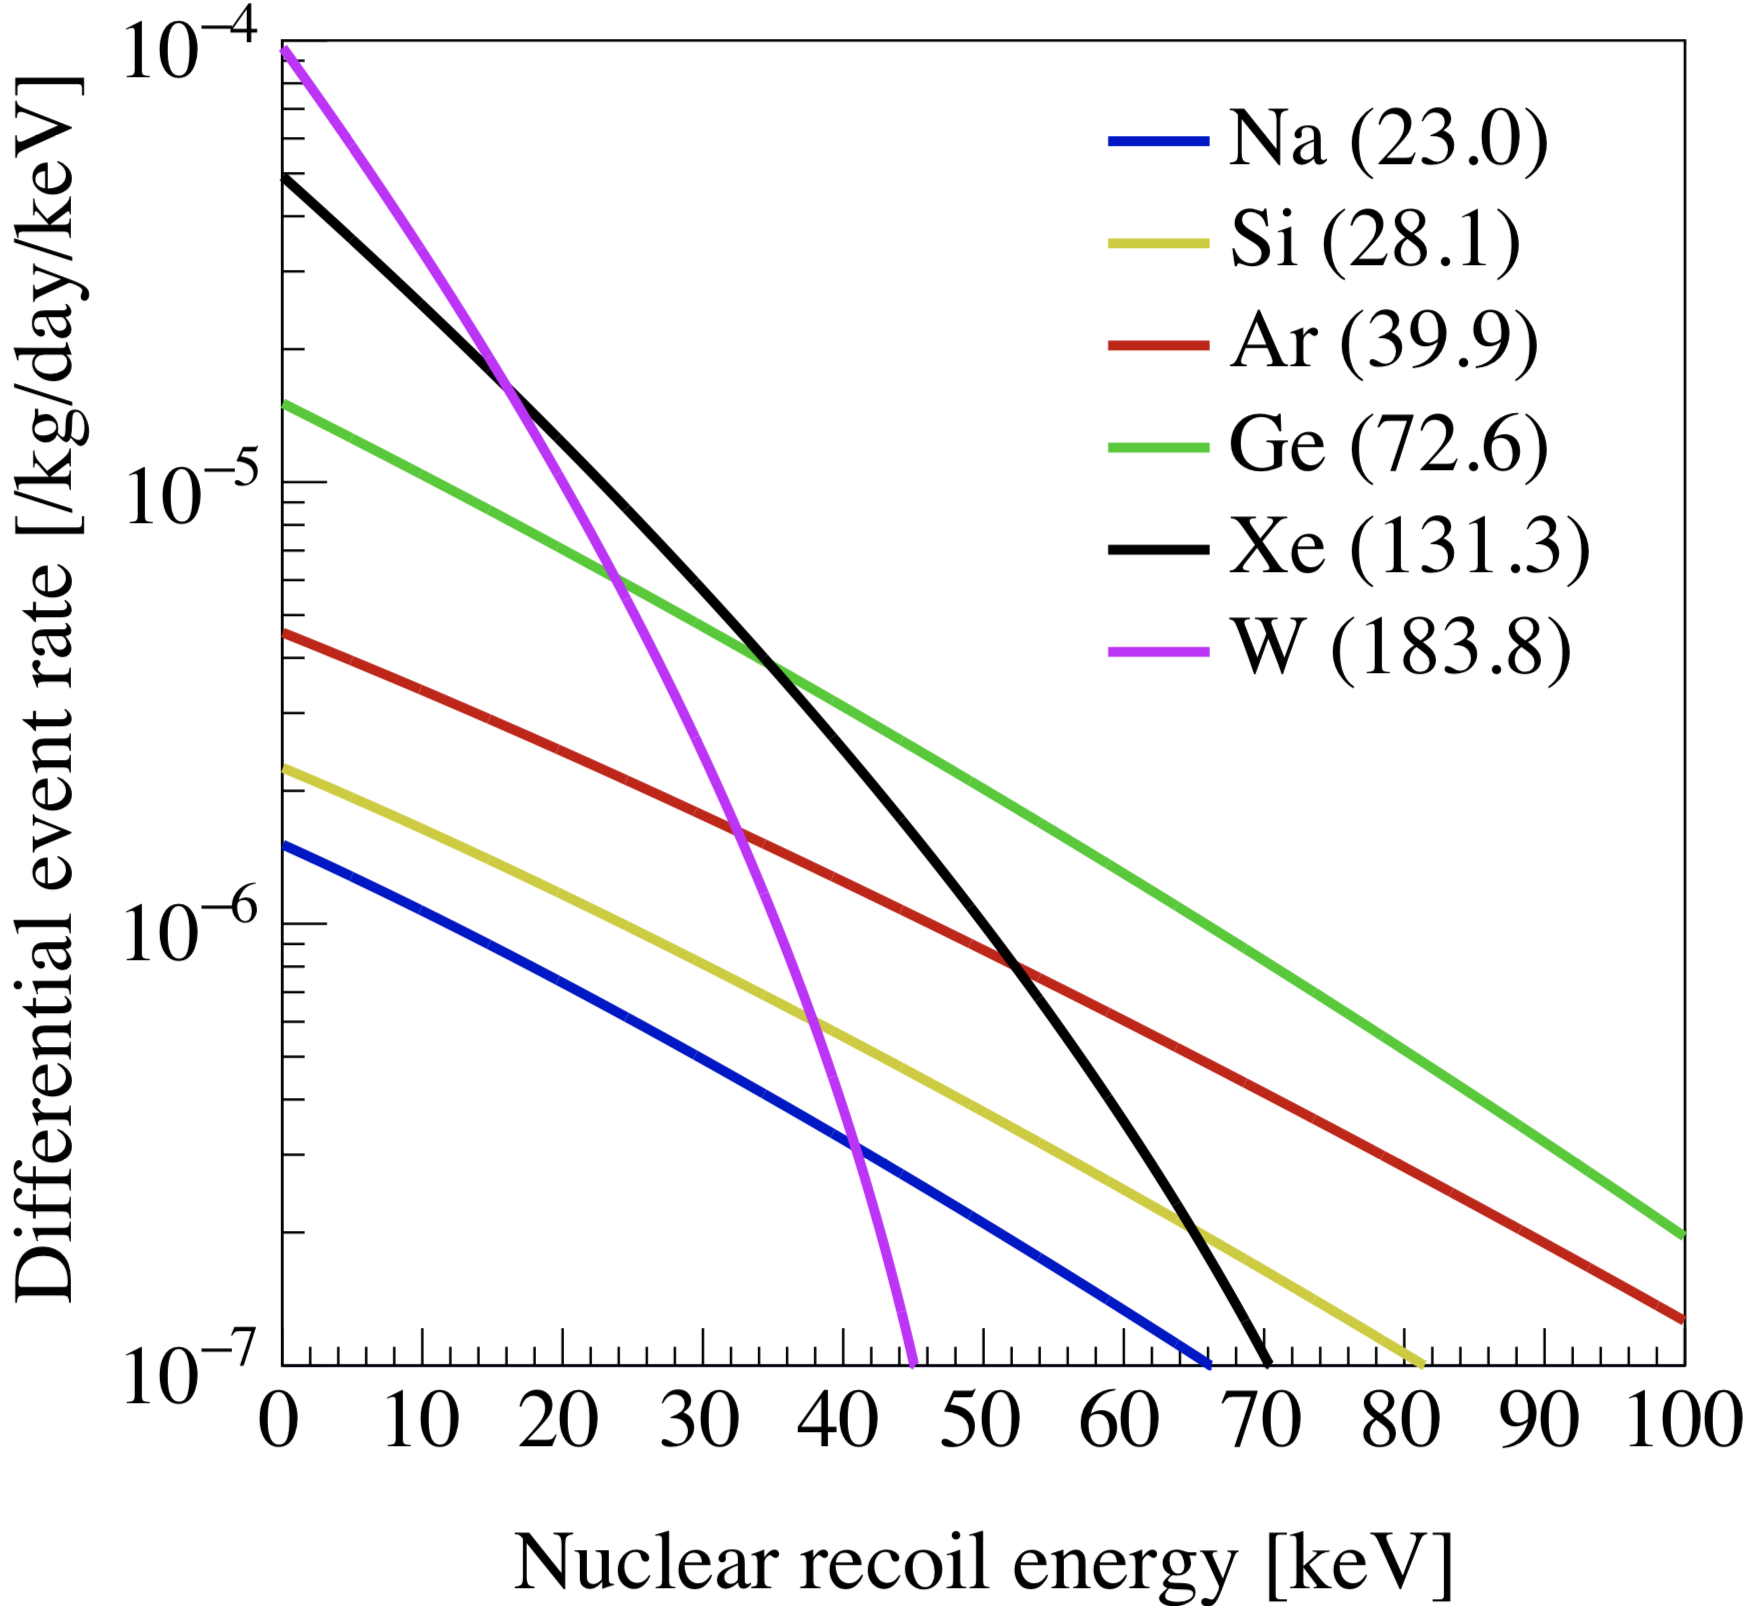
\includegraphics[scale=0.30]{Chapter_2/Figures/SI_nuclear_recoil_rates.png}
        \caption[Comparison of differential event rates of a $100 \; \MathText{GeV/c}^{2}$ WIMP interaction with several different target material, for an assumed cross-section of $\sigma^{SI}_{N} = 1 \; \MathText{zb}$]%
        {Comparison of differential event rates of a $100 \MathText{ GeV/c}^{2}$ WIMP interaction with several different target material with an assumed WIMP-nucleon cross-section of $\sigma^{SI}_{N} = 1 \; \MathText{ zb}$. The averaged atomic mass of each target element at natural abundance is indicated next to its symbol in the legend. Figure adapted from \cite{ibles}.}
        \label{fig:nuclear_recoil_rates}
        \end{center}
\end{figure}
%

The interactions taking place inside the TPC generate three types of signals, of which two can be read out by detectors alike. The first of these are the scintillation photons that are produced in the LXe volume via a mechanism that allows these photons to propagate through the liquid and be detected by VUV-sensitive PMTs that cover the top and bottom of the TPC. The interaction also produces ionisation electrons that are drifted upwards via a vertical electric field of several $100 \MathText{ V/cm}$. Once they reach the liquid surface, these electrons are extracted and accelerated through the gaseous phase, producing electroluminescence light, which is detected by the PMTs. The following sections will cover in detail the mechanisms in which these signals are produced and how they lead to a precise 3D position reconstruction and an effective background discrimination. 


%%------------------------------$$
%%------------------------------$$
\section{Particle Interactions \& Detection in a Dual-Phase Xenon TPC}
\label{sec:xenonphysics}

Interactions of particles inside a xenon TPC result in electron and nuclear recoils. The majority of the backgrounds originating from radioactive isotopes, such as beta or gamma particles interact mostly via electron recoils, leading to a significant ER rate. Neutral particles, such as neutrons or WIMPs are expected to undergo nuclear recoils. Electron recoils are interactions in which the incoming particle interacts with the orbital electrons of the xenon atoms, whereas nuclear recoils are kinetic interactions off of the atomic nucleus. The recoiling particles in both cases deposit their energy through multiple short-ranged interactions, forming a track in which a cascade of interactions take place. The end result of this cascade converts the initial particle energy into scintillation photons, ionisation electrons and atomic motion (heat), latter of which is undetectable by current TPCs. The following sections will discuss in detail the mechanisms of energy transfer and signal production in such interactions.

%%------------------------------$$
\subsection{Primary Energy Transfer}
\label{sec:energy_transfer}

In rare gases, such as xenon and argon, the energy deposited by radiation is expanded into the production of a number of electron-ion pairs, $N_{ion}$, excited atoms, $N_{ex}$, and thermalised free electrons, known as sub-excitation electrons liberated in the ionisation process. The deposited energy, $E_{0}$, can be expressed into ionisation, excitation, and sub-excitation electrons by the use of a Platzman equation \cite{Platzman, xenon_physics}:
%
\begin{equation} \label{eq:e_transfer}
    E_{0} = N_{ion}E_{ion} + N_{ex}E_{ex} + N_{ion}\eta,
\end{equation} 
%
where $E_{ion}$ and $E_{ex}$ are the mean ionisation and excitation energies, $N_{ion}$ and $N_{ex}$ are the number of ionised and excited atoms, and $\eta$ is the mean kinetic energy of ionised electrons. The energy required to produce a single electron-ion pair can be taken as an averaged value, defined as the W-value, where,
%
\begin{equation} \label{eq:w_value}
    W = E_{0}/N_{ion} = E_{ion} + E_{ex}(N_{ex}/N_{ion}) + \eta.
\end{equation} 
%
The average energy loss in ionisation is slightly larger than the ionisation potential or the band gap energy, resulting in the ratio of the W-value to that of ionisation potential or band gap to be 1.6-1.7 \cite{PhysRevA.48.1313}. In general, the W-value is smaller in the liquid phase, and in LXe, in comparison to liquid argon and neon. As a consequence, the ionisation yield in LXe is the highest of all noble liquids.

Although the above equation is believed to apply for electronic recoils, in the case of nuclear recoils, a large fraction of the deposited energy is spent in nuclear collisions, which do not result in either excitations or ionisations. Hence, an additional term may be considered in equation \ref{eq:e_transfer} to account for this loss. The ratio of $N_{ex}/N_{ion}$ has been measured to be $\sim0.2$ for electronic recoils and yields a value of $\sim1$ for nuclear recoils upon fitting to data \cite{xenon_physics, Dahl}. This difference in the initial ratio of exciton and electron-ion production is thought to be the underlying principle of discrimination between electron and nuclear recoils in two-phase TPCs. Further discussion on discrimination will follow in section \ref{subsubsec:recom_disc}.


%%------------------------------$$
\subsection{Primary Scintillation (S1)}
\label{subsec:s1}

The primary scintillation light---often referred to as an S1 signal---is produced via a process known as self-trapping, in which an excited xenon atom ($Xe^{\ast}$) forms a molecular dimer ($Xe^{\ast}_{2}$) with a neighbouring atom; the decay of which produces a VUV photon. Upon initial recoil, there are two distinct processes in particular that lead to S1 light production. The first of these are when an incoming particle creates an excited xenon atom, which leads to the creation and decay of an excited xenon dimer molecule \cite{xenon_physics}:
%
\begin{align} \label{eq:exciton_luminescence}
    &p_{i} + Xe \rightarrow Xe^{\ast} + p_{i}, \\
    &Xe^{\ast} + Xe \rightarrow Xe^{\ast, v}_{2}, \\
    &Xe^{\ast, v}_{2} + Xe \rightarrow Xe^{\ast}_{2} + Xe, \\
    &Xe^{\ast}_{2} \rightarrow  Xe +  Xe + \gamma,
\end{align}
%
where $p_{i}$ is the incoming particle, representative of any of the primary particle candidates present in such detectors, i.e., electrons, gamma rays, neutrons and so on. The superscript $v$ is used to distinguish vibrationally excited states from purely electronic excitation. The de-excitation of a vibrational state is mostly non-radiative but emission of infrared photons are also possible. The process detailed above is often referred to as \textit{exciton luminescence}.

An alternative process to exciton luminescence is \textit{recombination luminescence}. Although the end result of this process is identical to that of the process above, the initial interaction results in an ionised xenon atom, which undergoes recombination:
%
\begin{align} \label{eq:recombination_luminescence}
    &p_{i} + Xe \rightarrow Xe^{+} + p_{i} + e^{-}, \\
    &Xe^{+} + Xe + Xe \rightarrow Xe^{+}_{2} + Xe, \\
    &Xe^{+}_{2} + e^{-} \rightarrow Xe^{\ast\ast} + Xe, \\
    &Xe^{\ast\ast} + Xe \rightarrow Xe^{\ast} + Xe + (heat), \\
    &Xe^{\ast} + Xe \rightarrow Xe^{\ast, v}_{2}, \\
    &Xe^{\ast, v}_{2} + Xe \rightarrow Xe^{\ast}_{2} + Xe, \\
    &Xe^{\ast}_{2} \rightarrow  Xe +  Xe + \gamma.
\end{align}
%
The emission spectrum of the VUV scintillation photons originating from these two processes are similar as they share a common final stage. In a single event, both of these processes contribute in creating the summed S1 pulse---the collection of the VUV photons originating from an interaction site. However, it is important to note that the rate of recombination luminescence is heavily dependent on the initial energy recoil and more importantly, the electric field applied \cite{Dahl}. Application of an electric field serves as a mechanism to drift away any free electrons from the interaction site, hence suppressing recombination luminescence. 

Although there exists a probability for an optical transition of the excited atoms to undergo a transition to the ground state, the collision rates in liquid xenon often result in the formation of strongly bound two-atomic xenon molecules. These molecules are only bound in their excited states and can exist either in a single state, $^{1}\Sigma^{+}_{u}$, or a triplet state, $^{3}\Sigma^{+}_{u}$, thereafter transitioning to the repulsive ground state, $^{1}\Sigma^{+}_{g}$, where the two molecules separate into two neutral xenon atoms and emit a VUV photon centered at $\sim 178 \; \MathText{nm}$ \cite{FUJII2015293}. Thus, there is no re-absorption of the emitted photon, making xenon highly transparent to its own scintillation light---an important feature for a scintillator. The decay time constants of singlet and triplet states are very short, roughly 2.2 ns and 27 ns, respectively \cite{xenon_physics}. But recombination as highlighted in equation \ref{eq:recombination_luminescence} is a slow process and can impact the shape of the S1 pulse by adding a non-exponential third component, besides the fast (singlet decay) and the slow (triplet decay) components. The application of an electric field usually serves to reduce this third component by extracting the free electrons, hence suppressing recombination.

Furthermore, particle interactions at high energies ($\geq{}\MathText{MeV}$), such as $\alpha$-particles, can lead to the emergence of higher order processes that can decrease the number of primary scintillation photons. At these energies, the particle tracks formed due to high linear energy transfer (LET) increases the density of excited xenon atoms, thereby increasing the probability of interaction between two exited atoms. This process often leads to an increase in the ionisation rate in the track via a process called \textit{bi-excitonic quenching} \cite{bi_excitonic}, where
%
\begin{equation} \label{eq:bi-excitonic_quenching}
    Xe^{\ast} + Xe^{\ast} \rightarrow Xe^{+} + Xe + e^{-},
\end{equation} 
%
A similar process dubbed as \textit{penning ionisation} can also take place if a single excited xenon atom has enough energy to ionise a neutral xenon atom from the ground state
\cite{Dahl}, where
%
\begin{equation} \label{eq:bi-excitonic_quenching}
    Xe^{\ast} + Xe \rightarrow Xe^{+} + Xe + e^{-}.
\end{equation} 
%
In such processes, the excited xenon atoms have enough kinetic energy to ionise another atom upon a collision. These processes on average usually lead to the suppression of the summed S1 pulse at higher energy recoils, as the process reduces the probability of exciton luminescence, which often leads to the creation of a VUV photon.


%%------------------------------$$
\subsection{Ionisation \& Secondary Scintillation (S2)}
\label{subsec:s2}

The electrons which escape recombination are drifted up by a vertical electric field, effectively removing the electrons from the interaction site. The drift velocity of the electrons depend on the strength of the applied electric field. For liquid xenon, a field strength of $\sim 1 \; \MathText{kV/cm}$ can lead to a $2.25 \; \MathText{mm/\mu{}s}$ drift velocity. After about $10 \; \MathText{kV/cm}$, this dependence no longer holds and the drift velocity saturates at $\sim2.8 \; \MathText{mm/\mu{}s}$ \cite{e_drift}. An accurate understanding of the drift velocity and hence the applied electric field is important in reconstructing the depth (\textit{z} or the \textit{t} axis) at which the interaction took place, as this is proportional to the time difference between the S1 signal and the S2 signal---or put it another way, the time it takes for the electrons to travel to the surface of the liquid, as depicted in figure \ref{fig:tpc_diagram_cad}.

The ionisation electrons drifting in a TPC will also experience diffusion in all three spacial dimensions. Diffusion taking place across the \textit{x-y} plane dubbed as transverse diffusion, $D_{T}$, and the \textit{z} plane, also known as longitudinal diffusion, $D_{L}$. The transverse diffusion usually has no first-order effect on the shape of the summed S2 pulse, whereas despite being an order of magnitude smaller, where $D_{L}/D_{T} \simeq 0.1$, the longitudinal diffusion in LXe has a critical effect on the S2 shape as it dictates the photon time of arrival at the photo-detectors. Hence modelling this accurately is crucial for realistic simulations of pulses and for the determination of the depth of the interaction.

Furthermore, electronegative molecules such as $O_{2}$, $H_{2}O$ and $N_{2}O$ can dramatically decrease the mobility of drifting electrons. These molecules can capture free electrons and form negative ions with extremely low mobility, resulting in drift velocities of a few mm/s at practical electric fields. The probability of a capture by such species depend on the concentration, the reaction rate constant and the path length of the electron as it drifts towards the anode. These species are usually present in sourced xenon and often outgas from detector material, constantly contaminating the LXe. Hence, the purification of liquefied rare gases to contaminant levels that are \mathcal{O}(ppb) or lower is of great significance, especially for events at lower energies.

In reaching the liquid surface, the electrons have to overcome a potential barrier to be extracted over into the gas phase. This process is energetically unfavourable and hence an electric field of several kV/cm is usually applied between a grid just below and just above the liquid surface. Upon extraction, the electrons are accelerated through the gaseous layer to sufficient energies to excite the gas atoms, thus produce secondary scintillation, also known as \textit{electroluminescence}. This process allows very high amplification gains to be achieved, where signals from a single electron to be detected. The mechanism in which secondary scintillation photons are produced is similar to that explained for primary scintillation. A schematic diagram of a toy TPC, highlighting signal generation from an S1 and an S2 signal is depicted in figure \ref{fig:tpc_diagram_toy}. 
%
\begin{figure}[hb!]
    \begin{center}
        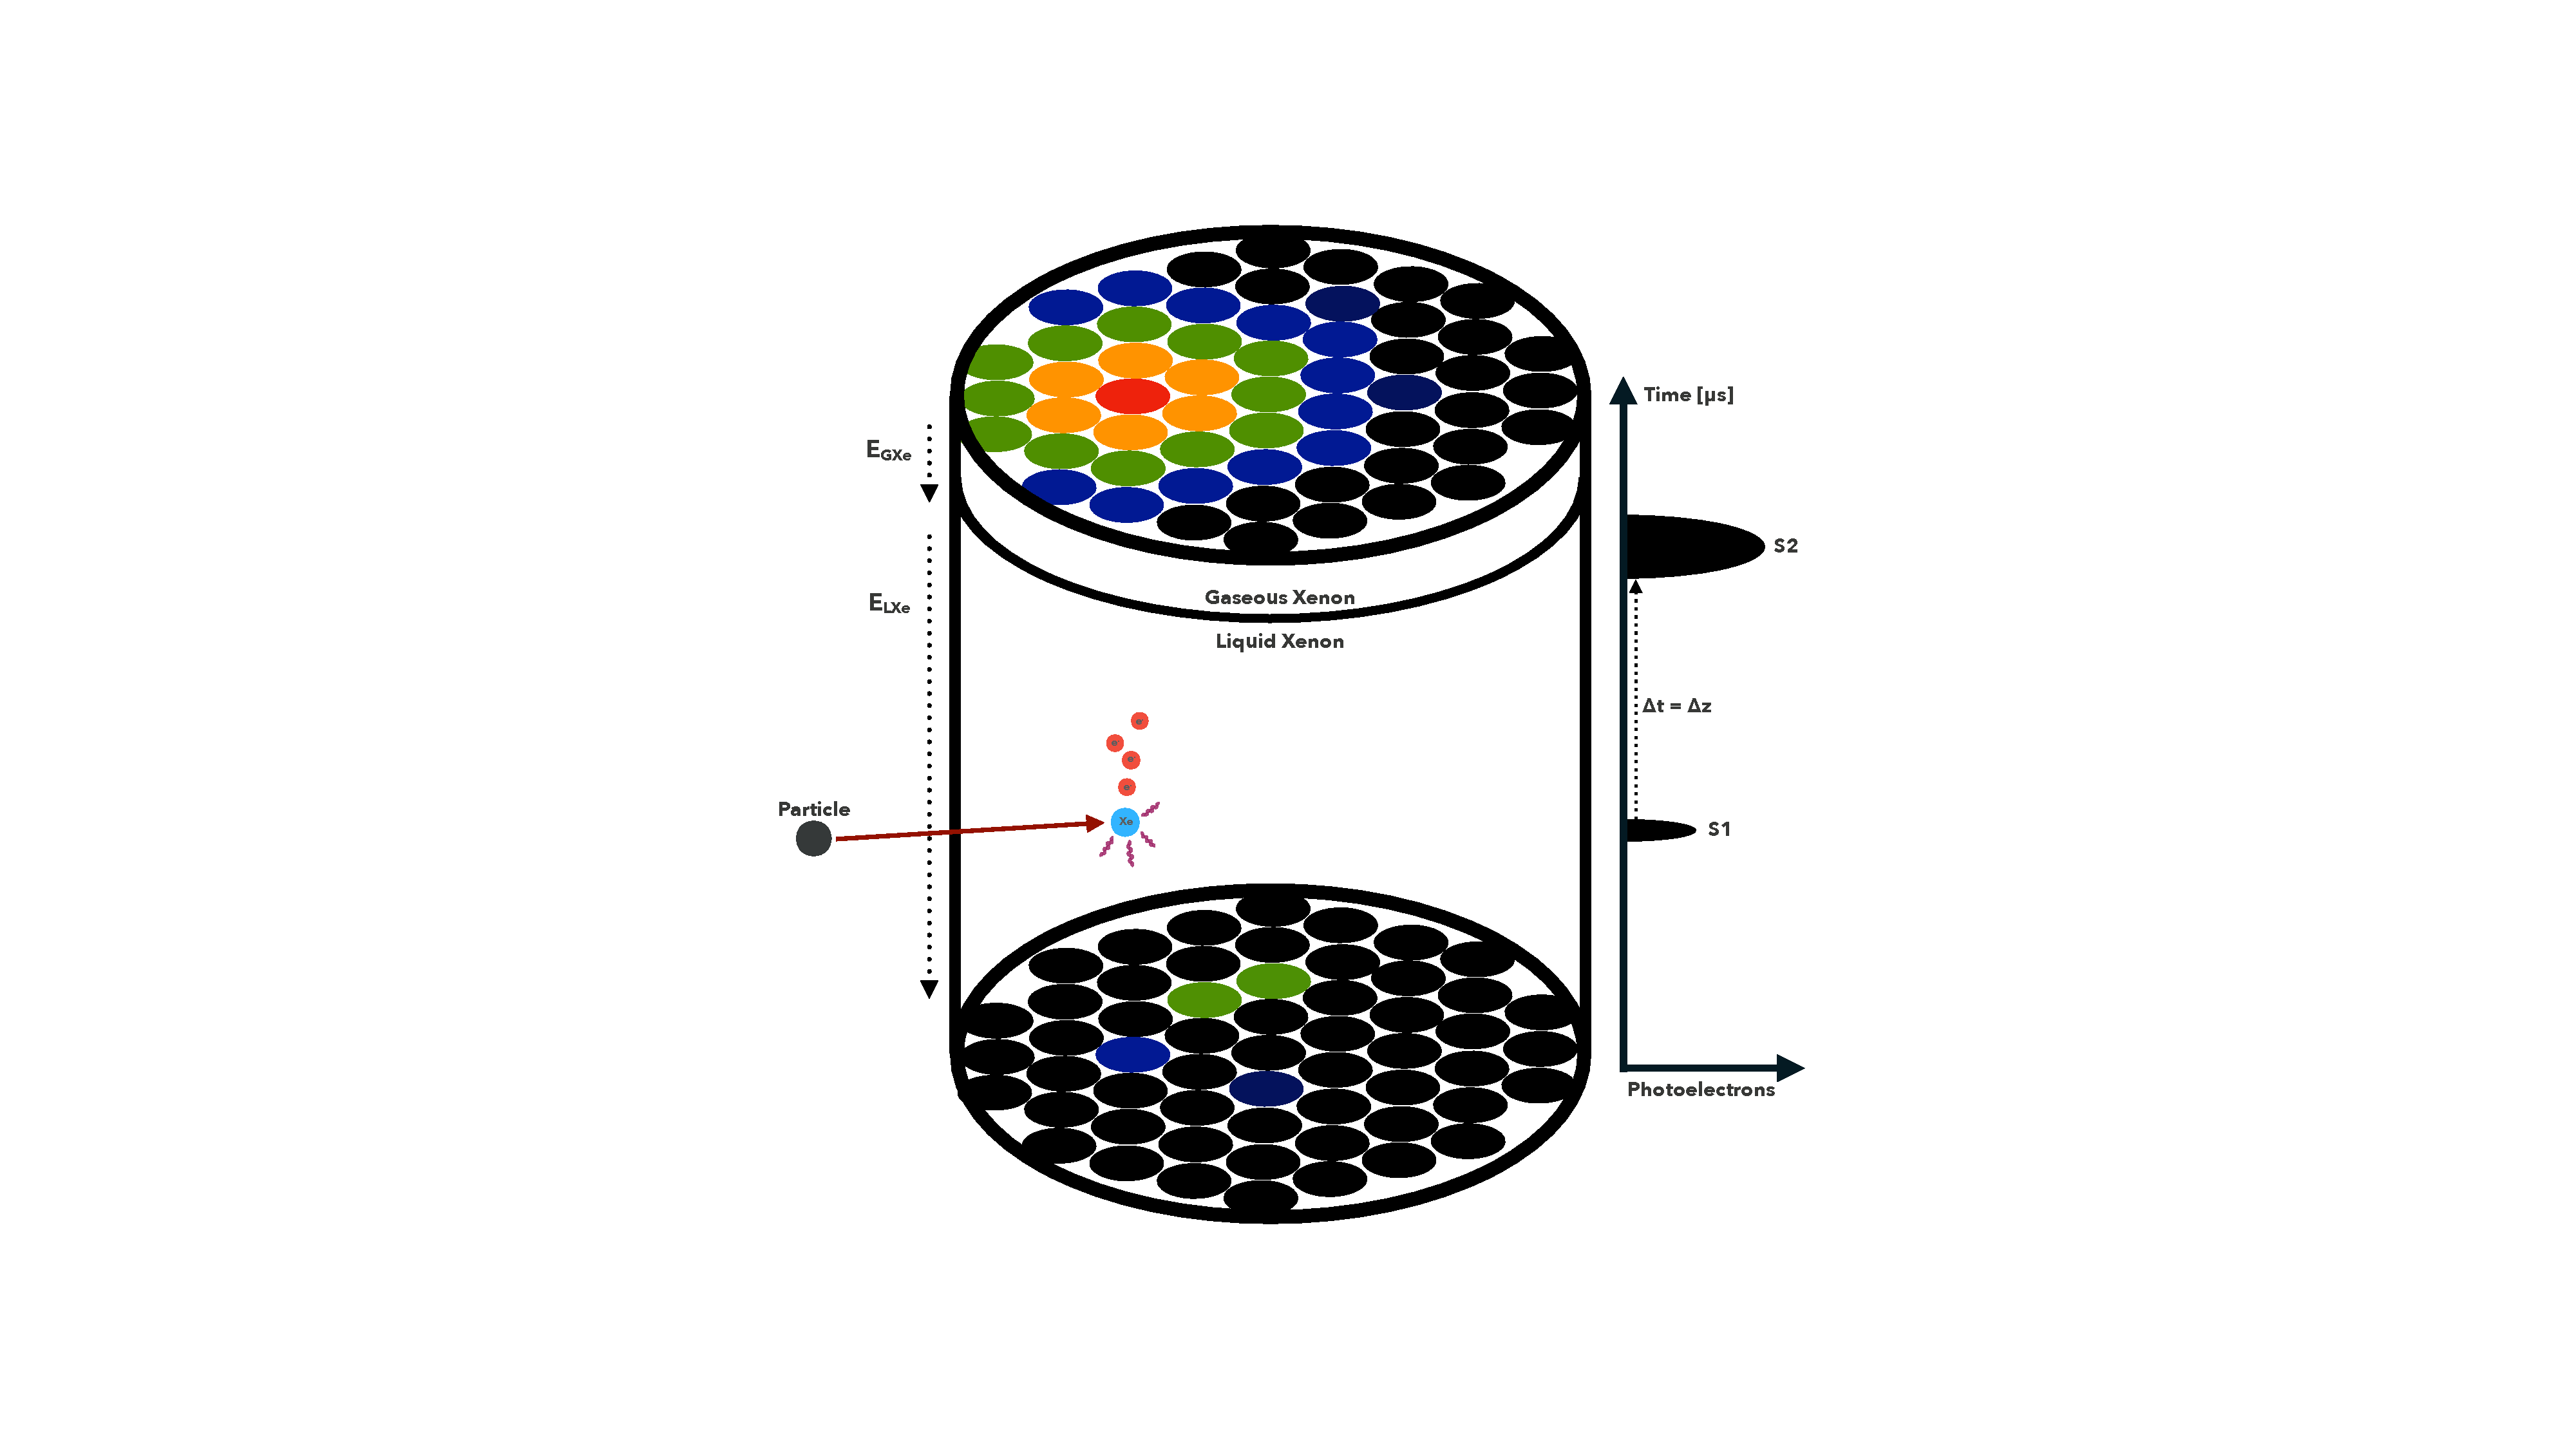
\includegraphics[scale=0.30]{Chapter_2/Figures/TPC_Diagram.pdf}
        \caption[Schematic of a single scatter event inside a dual-phase toy TPC, showing the S1 signal production and the drift of free electrons towards the gas layer]%
        {Schematic of a single scatter event inside a dual-phase toy TPC, showing the S1 signal production and the drift of free electrons towards the gas layer. The top and the bottom of the TPC is covered by PMTs that eventually detect the VUV photons created both in the liquid and in the gas phase. The diagram also depicts how TPCs allows for a 3D position reconstruction; where z is determined by the drift time of electrons and x-y determined by the PMT hit pattern.}
        \label{fig:tpc_diagram_toy}
        \end{center}
\end{figure}
%


%%------------------------------$$
\subsection{Energy Reconstruction and Signal Yields}
\label{sec:energy_recon_signal_yields}

Although the underlying principles that go into S1 and S2 production are relatively trivial, the modelling of these processes and correlating the output signal from a detector to a set of initial conditions depicting reality is less so. Taking into account the above, the number of emitted VUV photons, $n_{\gamma}$, and the escaped electrons, $n_{e}$, from an interaction site after recombination can be expressed as,
%
\begin{equation} \label{eq:photon_electron_recombination}
    &n_{\gamma} = N_{ex} + rN_{ion}, \\
    &n_{e} = (1 - r)N_{ion},
\end{equation}
%
where $N_{ex}$ and $N_{ion}$ are the total number of excited and ionised xenon atoms prior to recombination, respectively, and $r$ is the probability of recombination. In dual-phase TPCs, the detection of scintillation or ionisation due to a particle interaction is observed as an electronic signal that is proportional either to the number of emitted VUV photons, $S1 \propto n_{\gamma}$, or the number of escaped electrons, $S2 \propto n_{e}$. 

On an event-by-event basis, number of excitons, $N_{ex}$, and ionisations, $N_{ion}$, produced, is subject to statistical fluctuations---however, not independently. Therefore reconstructing the energy deposited by using only S1 or S2 light is also subject to the same fluctuations. In realising that, $ n_{\gamma} + n_{e} = N_{ex} + N_{ion}$, for any value of r, and the anti-correlation of S1 and S2 light, a linear combination of S1 and S2 could be used to construct a combined signal to form an improved energy estimator,
%
\begin{equation} \label{eq:combined_energy}
    E_{0} = \mathcal{L}W(n_{\gamma} + n_{e}). 
\end{equation}
%
The W-value in this case represents the average energy required to produce either an exciton or a electron-ion pair, and has an approximated value of 13.7 eV in LXe \cite{Dahl}. $\mathcal{L}$ is referred to as the \textit{quenching factor}, representing the fraction of the recoil energy that is transferred to electronic excitation instead of atomic motion. For electron recoils, this fraction is assumed to be negligible; whereas for nuclear recoils, a large amount of energy is lost as atomic motion. The commonly used model in estimating for this fraction comes from Lindhard’s theory, which is based on heavy ion quasi-elastic collisions and gives the energy dependent nuclear recoil quenching factor as \cite{Lindhard, Lindhard_2},
%
\begin{equation} \label{eq:combined_energy}
    \mathcal{L} = \frac{kg(\epsilon)}{1 + g(\epsilon)},
\end{equation}
%
where $k$ is a constant of proportionality between electronic stopping power and the recoil velocity of the nucleus and $g(\epsilon)$ is a function that models the ratio of electronic-to-nuclear stopping powers. $\mathcal{L}$ is sometimes referred to as the \textit{Lindhard factor} and the energies corresponding to ER or NR events are commonly reported as $keV_{ee}$ and $keV_{nr}$, highlighting the electronic and nuclear recoil equivalent energies.

\subsubsection{Light \& Charge Yields in Liquid Xenon}
\label{subsubsec:light_charge}

In a xenon TPC, where searches are conducted across a wide range of recoil energies, it is often useful to define the light, $L_y$, and charge, $Q_y$, yields, as the number of photons emitted in scintillation or the number of electrons ionised, per keV of recoil energy, respectively, where
%
\begin{equation} \label{eq:combined_energy}
    &L_y = n_{\gamma}/E_{0}, \\
    &Q_y = n_{e}/E_{0}.
\end{equation}
%
The prediction of the liquid xenon yields under the assumed drift electric fields of 180 V/cm and 310 V/cm are presented as the dashed and solid lines in figure \ref{fig:light_charge_yields}. These electric fields are highlighted in particular to represent the fields operated by the LUX experiment and that which the LZ experiment aims to operate under, respectively. The figure also overlays measurements made by the LUX and the PIXeY experiments for both electron and nuclear recoils, down to a few keV of recoil energy, showing a good agreement with the predictions from NEST (Noble Element Simulation Technique) \cite{Szydagis_2011, Mock_2014}. NEST is a simulation package developed as an extension to \textsc{Geant4} \cite{Geant4} to simulate the non-linear behaviour of the energy dependence of scintillation and charge yields as seen by liquid noble detectors. Under its hood, NEST can be seen as a collection of models and approximations that predict the light and charge yields of noble gas elements as a function of recoil energy, electric field, particle type, temperature and pressure. A new version of the \textsc{NEST} software package was released in 2018 (v2.0.0) \cite{nest_v2}, moving away from the initially proposed semi-empirical models, towards a more data-driven approach to match the extensive collection of global data that exists. 

The anti-correlation of light and charge yields for both electron and nuclear recoils are apparent from the solid and dashed \textsc{NEST} lines. The increased recoil energy under a fixed electric field, yields in more ionised electrons, increasing the probability of recombination, and hence increases the light yield. Furthermore, the quanta produced per keV of deposited energy for NR interactions are shown to be quenched across the same energy range. The figure also shows a subtle but noticeable difference between the yields as predicted for 180 V/cm and 310 V/cm; the larger field reduces the recombination probability for both ER and NR events, resulting in a larger charge yield across the energy range.
%
\begin{figure}[hbt!]
    \centering
    \begin{subfigure}
        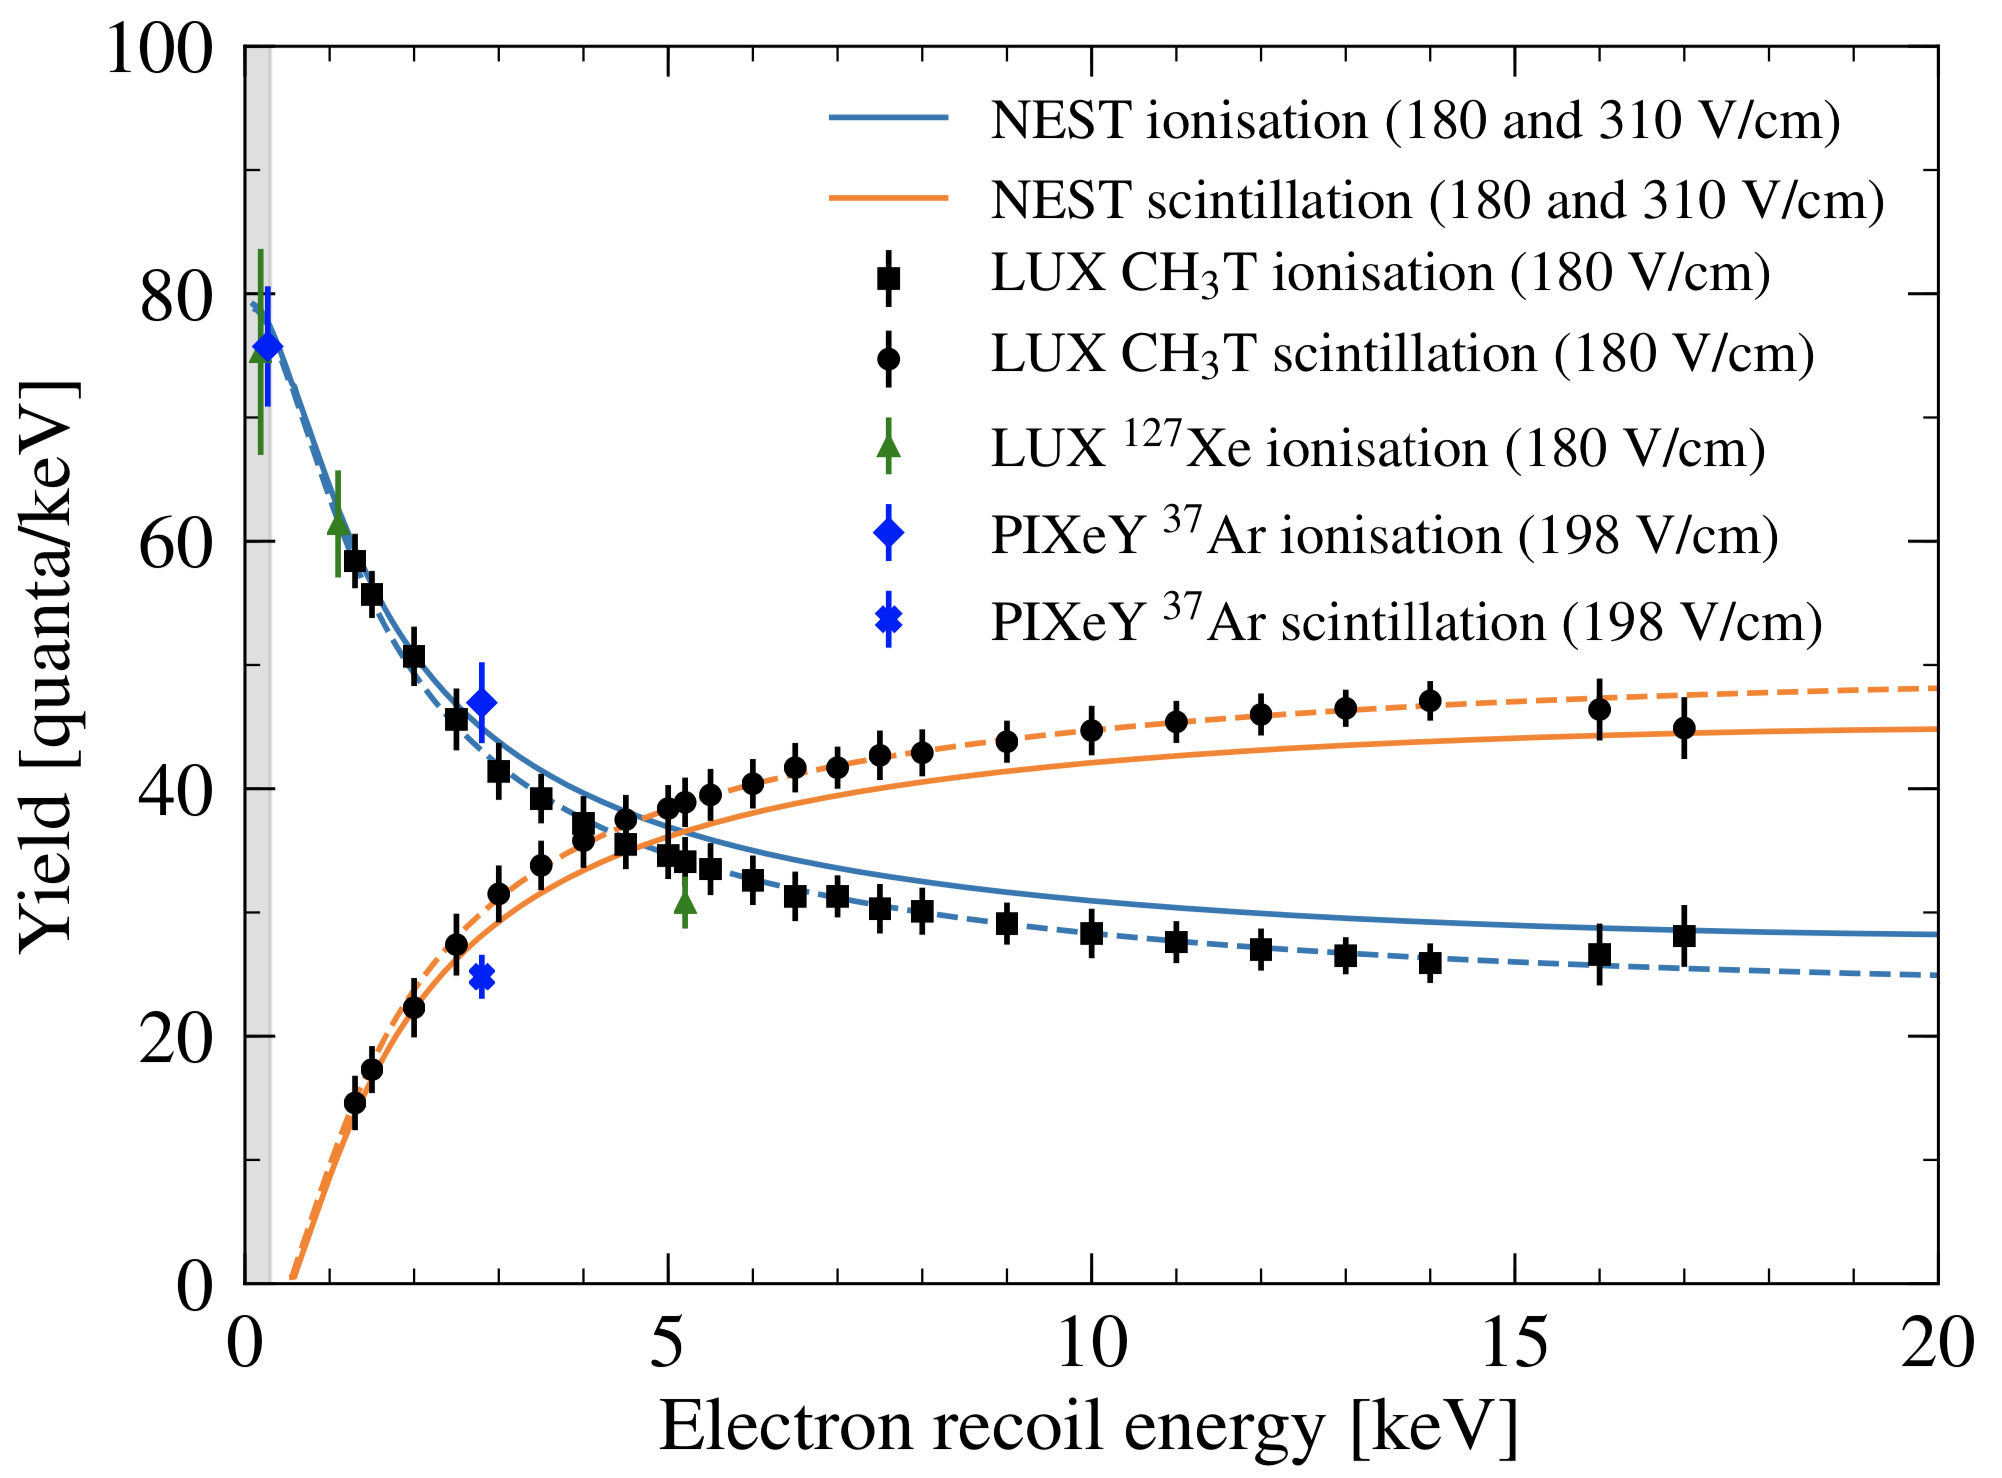
\includegraphics[scale=0.22]{Chapter_2/Figures/electron_recoil_yield.png}
    \end{subfigure}
    \begin{subfigure}
        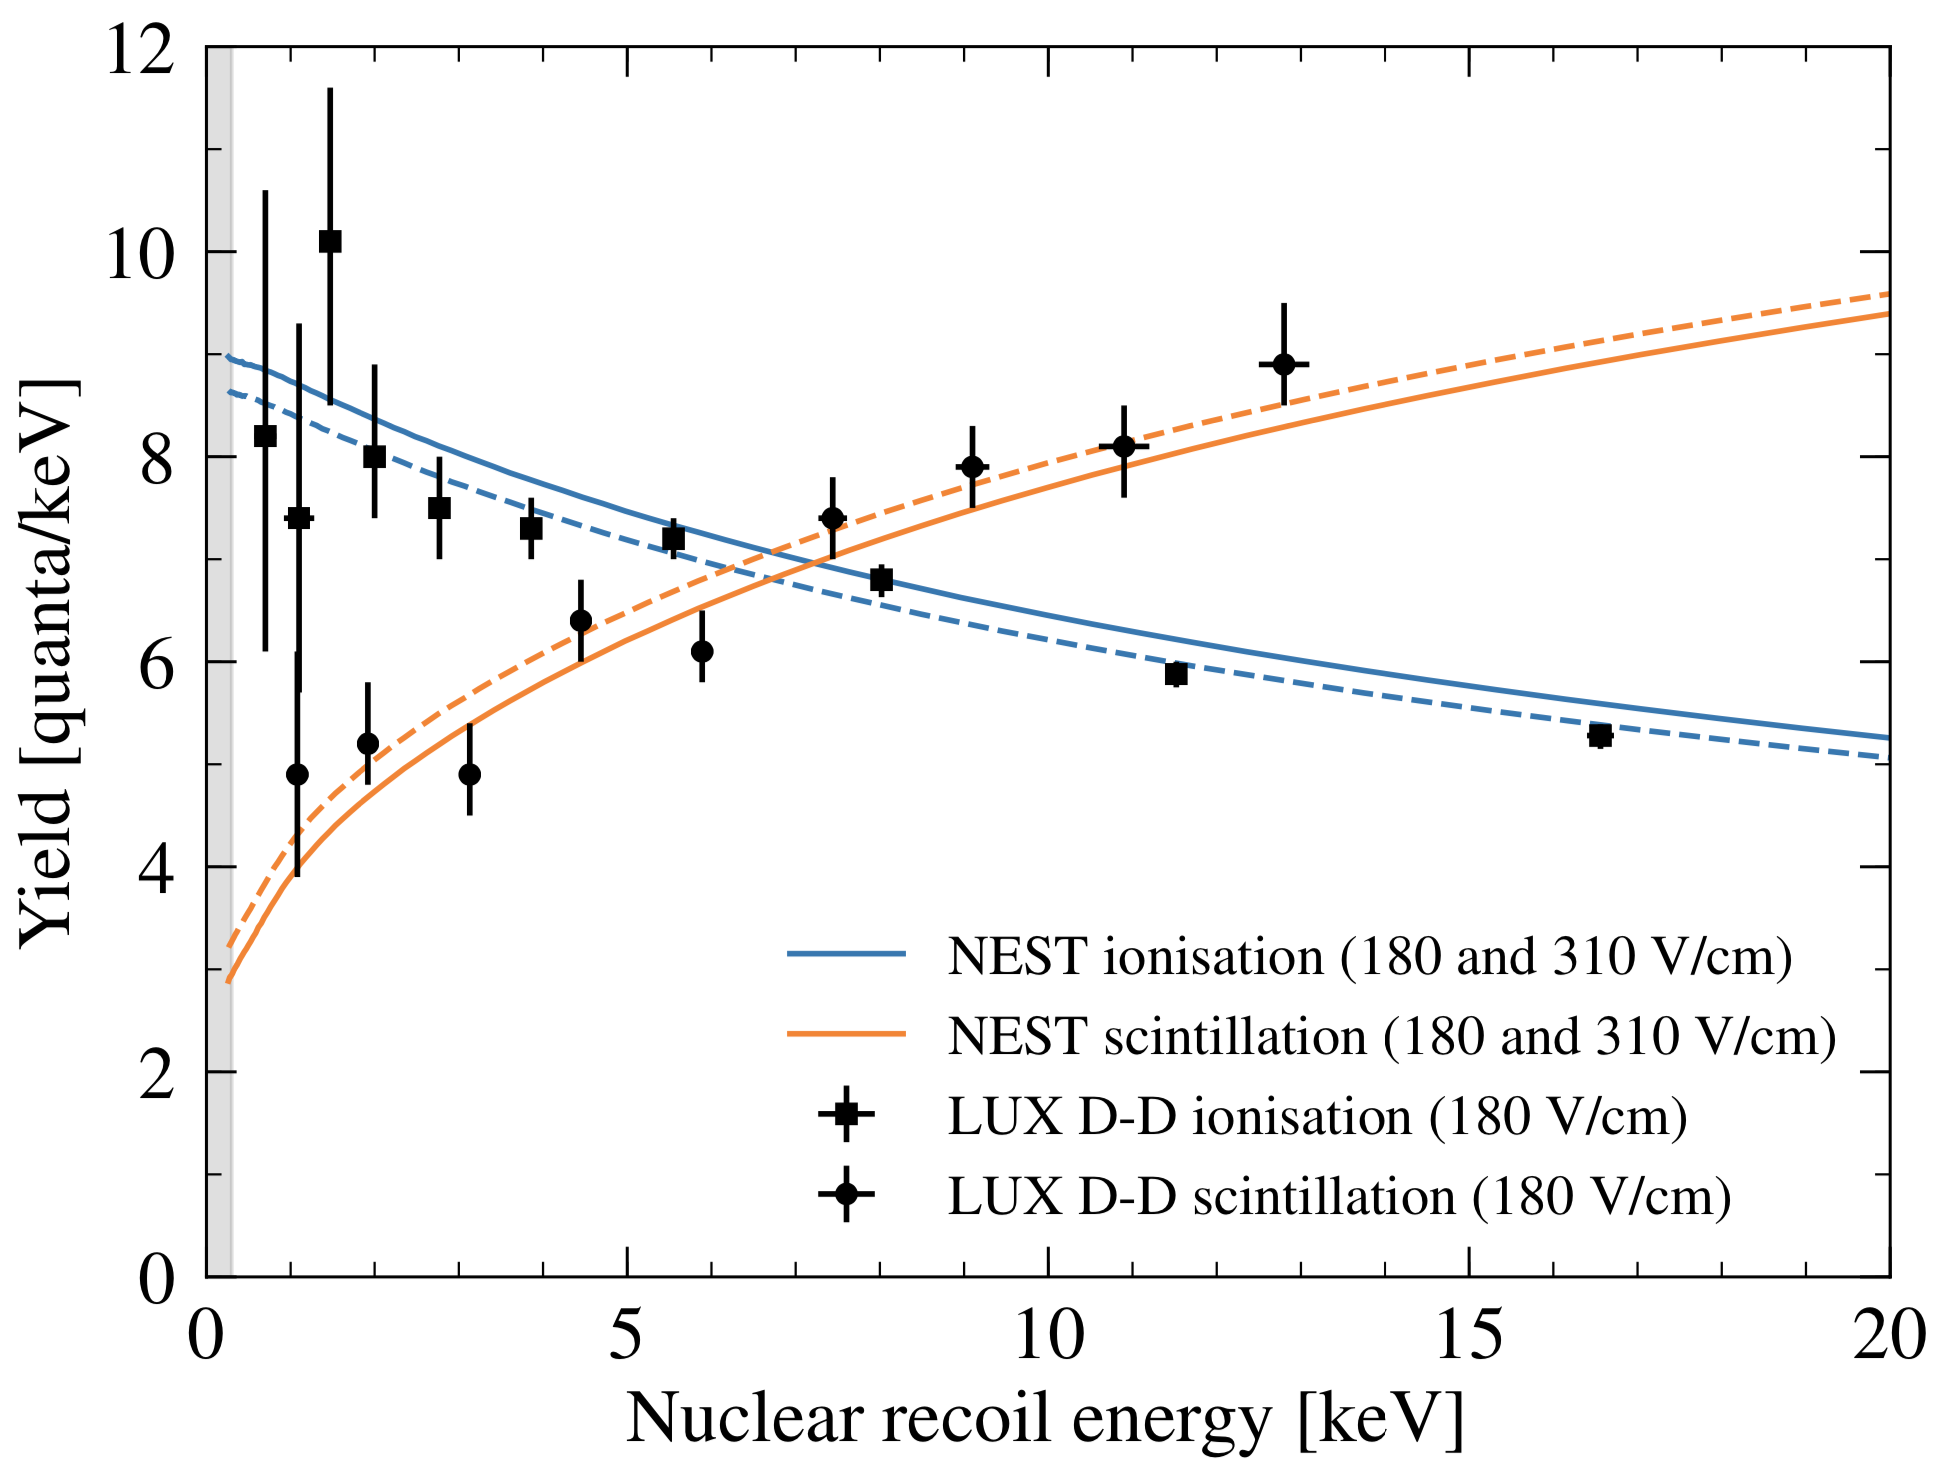
\includegraphics[scale=0.22]{Chapter_2/Figures/nuclear_recoil_yield.png}
    \end{subfigure}
    \vspace*{-5mm}
    \caption[Liquid xenon scintillation and ionisation yields for electron recoils and nuclear recoils.]%
    {Liquid xenon scintillation and ionisation yields for electron recoils (left) and nuclear recoils (right). The NEST prediction of the scintillation and ionisation yields at drift electric field of 180 V/cm (dashed) and 310 V/cm (solid) are represented as the orange and blue lines, respectively. Measurements from LUX CH$_{3}$T \cite{lux_tritium} and $^{127}$Xe \cite{lux_low_energy_cal} calibrations, along with the PIXeY $^{37}$Ar source measurements \cite{PIXeY} are overlaid. Figure adapted from Ref. \cite{ibles}.}
    \label{fig:light_charge_yields}
\end{figure}
%

\subsubsection{Combined Energy Scale}
\label{subsubsec:combined_energy}

The reconstruction of deposited or recoil energy as seen by the detector has to take into account detector specific efficiencies. Upon creation, a single VUV photon will reflect off of surfaces many times, before being successfully recorded by a PMT. The inefficiencies in this process, i.e., absorption of photons upon reflection, the quantum efficiency of PMTs, etc., serves to reduce the overall S1 size. Similarly, inefficiencies for the S2 light is also present, i.e., presence of electronegative molecules, efficiency of extraction into gas phase, etc., reduces the overall S2 size. Therefore, true S1 and S2, as seen by the detector can be defined as,
%
\begin{equation} \label{eq:photon_electron_recombination}
    &S1 = g_{1}n_{\gamma}, \\
    &S2 = g_{2}n_{e}.
\end{equation}
%
Here $g_{1}$ represents the total light collection efficiency in liquid and $g_{2}$ represents the electron detection efficiency, which can be further represented as $g_{2}=N_{ph}\epsilon{}g_{1(gas)}$, where $\epsilon{}$ is the electron extraction efficiency, $N_{ph}$ is the number of electroluminescence photons produced per electron, and $g_{1(gas)}$ is the light collection efficiency in the gas phase. By using the combined energy estimator defined in equation \ref{eq:combined_energy}, energy as reconstructed by a detector takes the form,
%
\begin{equation} \label{eq:combined_energy_detector}
    E_{0} = \mathcal{L}W\left(\frac{S1}{g_{1}} + \frac{S2}{g_{2}}\right). 
\end{equation}
%
Both $g_{1}$ and $g_{2}$ can be measured experimentally by the use of known calibration sources, as detailed in \cite{lux_signal_yields} for the LUX experiment. Due to the difference in the quenching factors between ER and NR events, calibration sources using \grays{}, are presented in electron equivalent energies, \kevee{}. As an example of the way these scales work, a \gray{} induced electron recoil of 6 \kevee{} would produce roughly the same total light and charge as a nuclear recoil of a $\sim30$ \kevnr{}.

\subsection{ER \& NR Discrimination}
\label{subsubsec:recom_disc}

As mentioned previously, electron and nuclear recoils tend to appear in different regions of the energy-space, as seen by dual-phase LXe detectors. The conventional way in which events are displayed in such detectors is to plot directly in S1-S2 space. An example of such a plot from the LUX calibration data is shown in figure \ref{fig:er_nr_discrimination} \cite{lux_signal_yields}. When plotting in log$_{10}$(S2/S1) verses S1 space, a clear band structure for ER and NR becomes apparent. The discrimination as seen in this plot is thought to be a consequence of the difference in energy dissipation mechanisms for ER and NR events, as energy is deposited into LXe. To first order, the discrimination originates from the ratio of $N_{ex}/N_{ion}$, where more excitons, for the same energy deposition, are expected to form for a NR than for an ER, hence pushing the NR band lower in the log$_{10}$(S2/S1) axis. The quantification of discrimination for LXe is conventionally taken as the fraction of ER events that leak below the NR mean, divided by the total ER events. Although discrimination varies across S1 or at higher energies, this quantity can be averaged in a desired energy range, i.e. WIMP region of interest. LZ is expected to reach an ER-NR discrimination of 99.5\%.
%
\begin{figure}[ht!]
    \begin{center}
        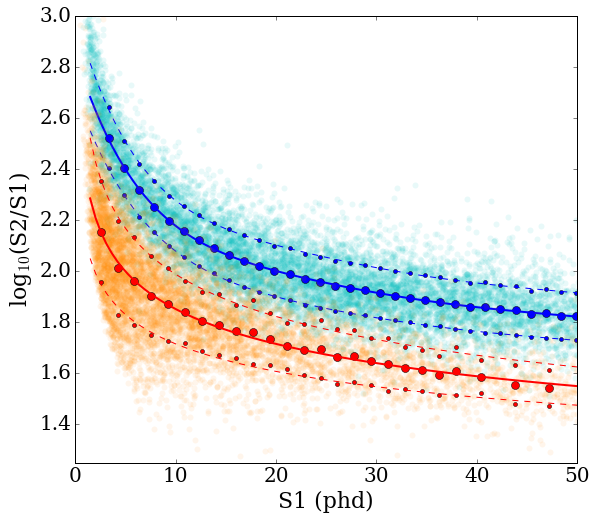
\includegraphics[scale=0.60]{Chapter_2/Figures/PAPER_logS2S1_ERNRBandData.png}
        \caption[Calibration data from the LUX experiment, highlighting the ER and NR band formations in the S1-S2 energy-space.]%
        {Calibration data from the LUX experiment, highlighting the ER and NR band formation (cyan and orange, respectively) in the S1-S2 space. Large filled circles show the fitted band Gaussian mean and small filled circles indicate the fitted Gaussian $\pm1\sigma$. Power law fits to the means and $\pm1\sigma$ are shown with solid and dashed lines \cite{lux_signal_yields}.}
        \label{fig:er_nr_discrimination}
    \end{center}
\end{figure}
%


%%------------------------------$$
\section{The LUX-ZEPLIN Experiment}
\label{sec:lz_detector}

The LUX-ZEPLIN dark matter experiment is housed in the Sanford Underground Research Facility (SURF) in Lead, South Dakota, USA. The detector design is inspired from the LUX and ZEPLIN---III experiments that independently operated dual-phase LXe detectors at much smaller scales \cite{LUX_experiment, zeplin3}. In search for WIMP dark matter, the LZ detector at its core will operate a dual-phase xenon TPC with an active mass of 7 tonnes. To achieve optimal sensitivity, the detector is placed 4850 feet underground inside a water tank; shielded from cosmogenic and atmospheric backgrounds. In operating a LXe skin veto system (dubbed as the skin veto) that surrounds the TPC, and additionally, an outer veto system---dubbed as the outer detector (OD), which utilizes a gadolinium-loaded liquid scintillator (GdLS), the LZ experiment is projected to exclude spin-independent WIMP-nucleon cross sections above $1.4 \times 10^{-48} \; \MathText{cm}^{2}$ for a $40 \; \MathText{GeV/c}^{2}$ WIMP mass at a 90\% confidence level \cite{akerib2018projected}. The following sections will detail the experimental design of LZ, highlighting key operational elements in its search for dark matter, some of which are displayed in figure \ref{fig:cross_sectional_LZ}.

%
\begin{figure}[ht!]
    \begin{center}
        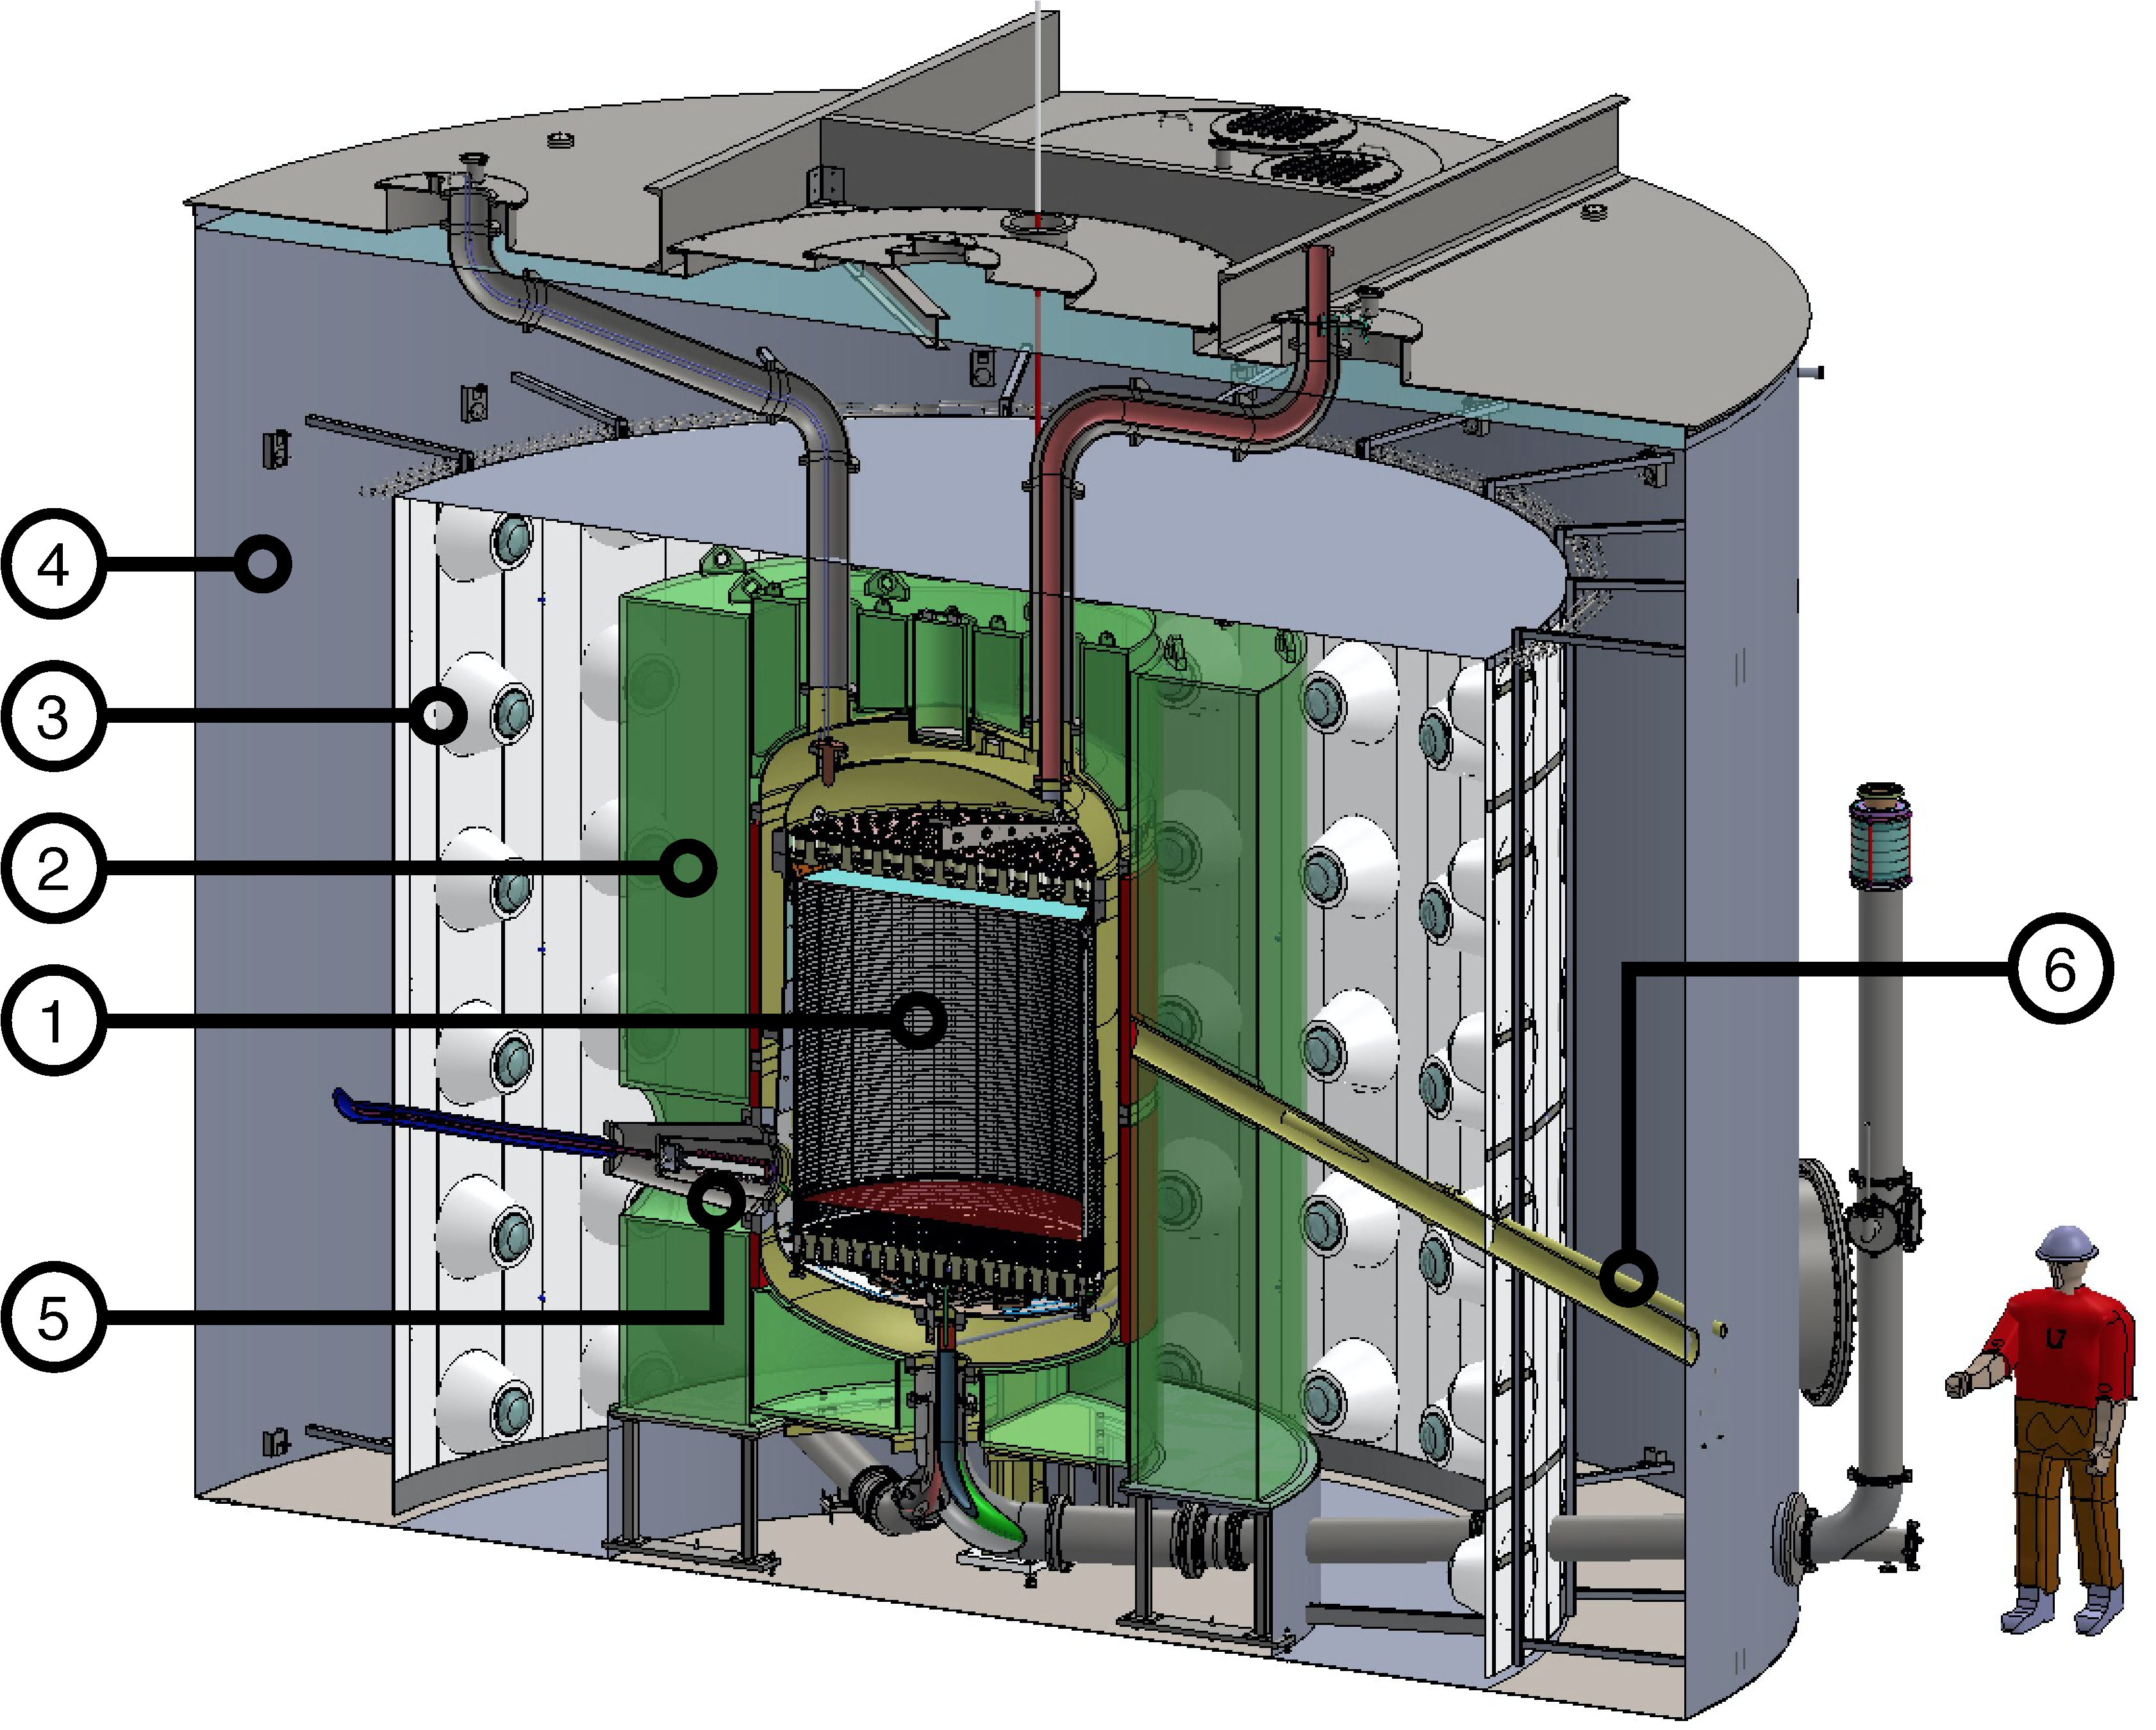
\includegraphics[scale=0.18]{Chapter_2/Figures/LZ_detector_cross_section.pdf}
        \caption[Cross-sectional CAD model of the LZ experiment, highlighting the major detector subsystems.]%
        {Cross-sectional cad model of the LZ experiment, highlighting the major detector subsystems. The LXe TPC (1) is located at the center with PMT arrays covering the top and the bottom. The TPC is sealed within a double-walled vacuum-insulated titanium cryostat that is surrounded by gadolinium-loaded liquid scintillator (GdLS) outer detector (2), surrounded by a suite of 8" PMTs (3) inside the water tank (4). The cathode high voltage (5) and the neutron calibration source conduit (6) are also depicted \cite{Akerib:2019fml}.}
        \label{fig:cross_sectional_LZ}
        \end{center}
\end{figure}
%

\subsection{Liquid Xenon TPC \& Skin Detector}
\label{subsec:tpc_skin}}

The xenon detectors operated by LZ are housed in a double-walled vacuum-insulated titanium cryostat. The inner cryostat vessel (ICV) contains within it the TPC and the skin region. In operation, LZ handles a total of 10 tonnes of liquid xenon; 7 tonnes held inside the TPC and an additional $\sim2$ tonnes held in the skin region. The TPC volume is usually referred to as the active volume which constitutes the WIMP target, and the skin volume refers to the region between the inner cryostat vessel and the outer surface of the TPC---both of which are instrumented with PMTs. 

The TPC volume measures approximately 1.5 m in diameter and height, with a primary objective of detecting S1 and S2 light that are produced both in the liquid and the gaseous layers of this volume. To optimise the collection efficiency of S1 light, the TPC walls as seen by the photons are coated by highly reflective PTFE with a reflectivity of $\geq97.3\%$ when immersed in LXe \cite{Neves_2017}. The S2 electrons produced within the liquid are handled by the operation of four horizontal electrode grids, woven from stainless steel wires, splitting the TPC into three different regions of electric field.

The drift field region (DFR) with a length of 145.6 cm extends from the cathode grid at the bottom of the detector, to the gate grid, located just below the liquid surface, and is shaped by 58 equally spaced titanium field-shaping rings that are embedded into the PTFE panels of the TPC wall. The DFR provides a vertical drift field for ionised free electrons to drift to the liquid surface. The extraction field region (EFR), also known as the electroluminescence region, is located between the gate (5mm below liquid surface) and the anode (8 mm into the gas). Electrons drifted to the surface of the liquid are extracted by this region and accelerated through the gas layer to generate $\sim$820 electroluminescence photons per electron, of which the S2 light is constructed. The final region, known as the reverse field region (RFR) is located between cathode and another grid that sits just below. This space uses 8 field-shaping rings and serves to protect the bottom PMT array from the high potential of the cathode grid, while also drifting the electrons created in this region downwards, hence removing the S2 signal from events occurring below the cathode. A diagram of the TPC with key highlights are shown in figure \ref{fig:tpc_diagram}.

%
\afterpage{
    \begin{figure}[h!]
        \centering
        \begin{subfigure}
            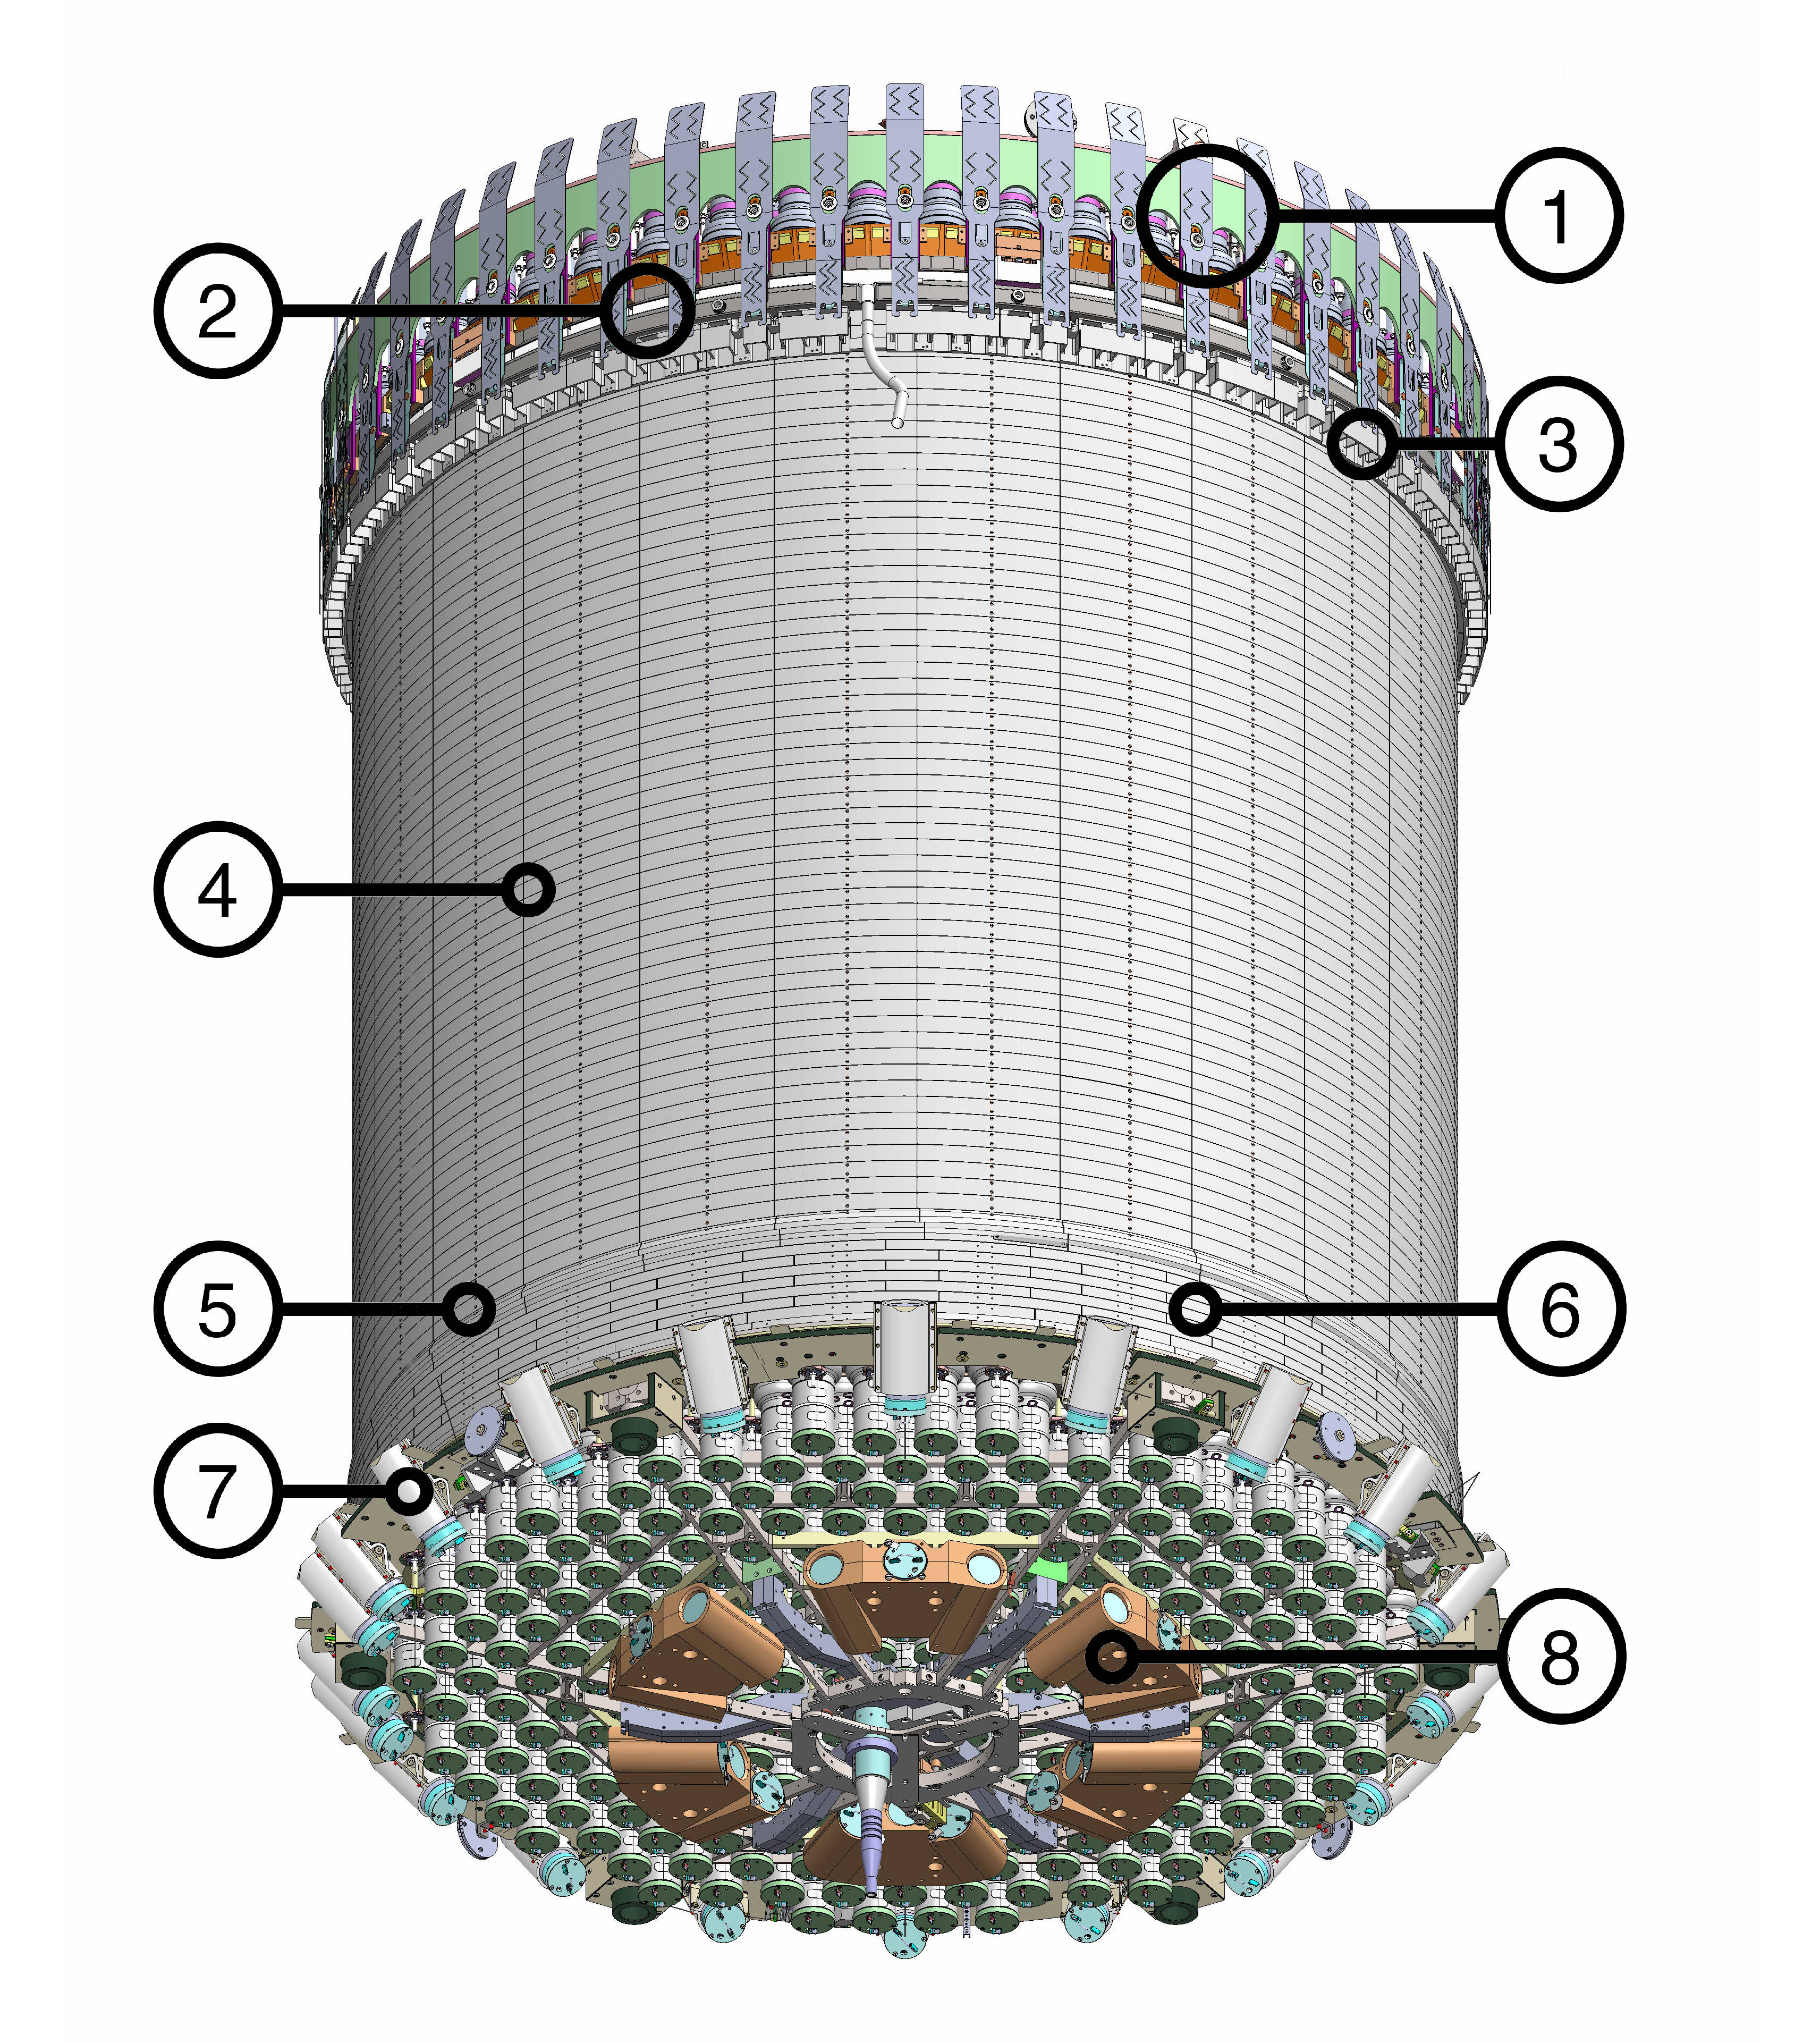
\includegraphics[scale=0.60]{Chapter_2/Figures/TPC_CAD_reduced.jpg}
        \end{subfigure}
        \hspace*{10mm}
        \begin{subfigure}
            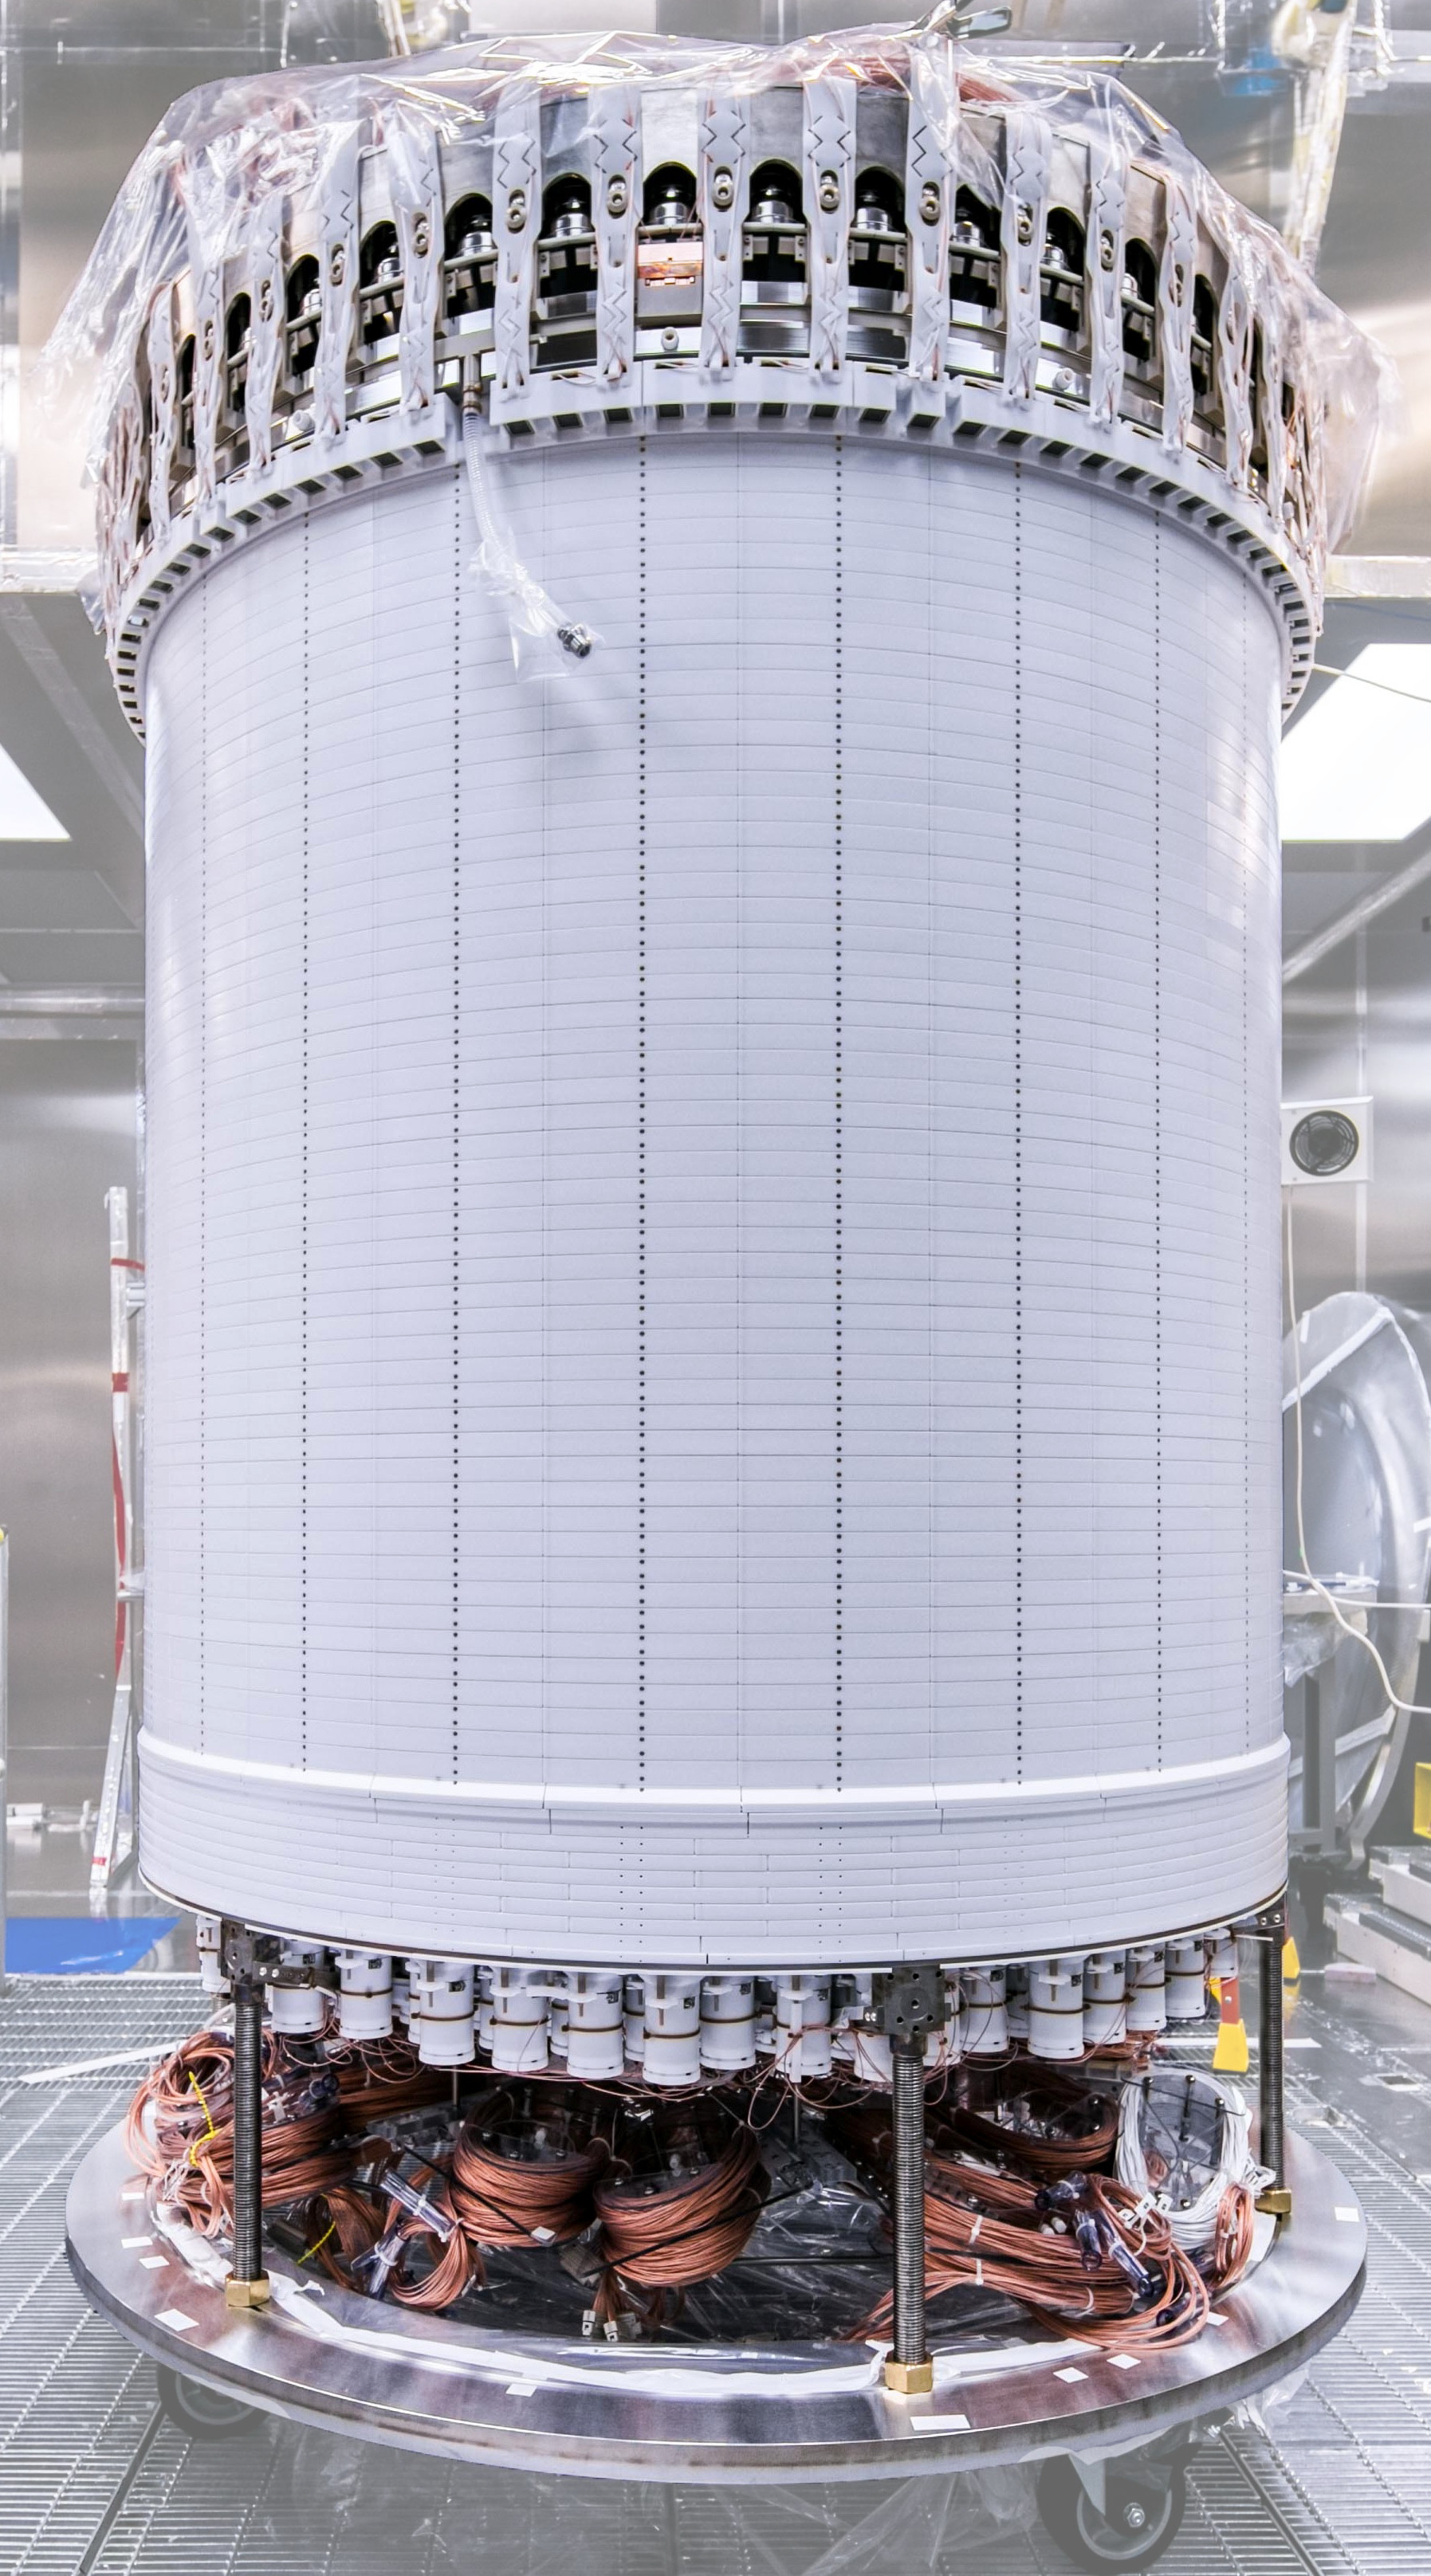
\includegraphics[scale=0.28]{Chapter_2/Figures/TPC_real_reduced.jpg}
        \end{subfigure}
        \caption[A diagram showing the CAD (left) and the fully constructed TPC (right), detailing the key components of the system.]%
        {A diagram showing the CAD (left) and the fully constructed TPC (right), detailing the key components of the system. 1- Top PMT array; 2-Gate-anode and weir region (liquid level); 3-Side skin PMTs (1-inch); 4-Field cage; 5-Cathode ring; 6-Reverse field region; 7-Lower side skin PMTs (2-inch); 8-Dome skin PMTs (2-inch). Photographed by Matthew Kapust, Sanford Underground Research Facility \cite{Akerib:2019fml}.}
        \label{fig:tpc_diagram}
    \end{figure}
    \begin{figure}[h!]
        \centering
        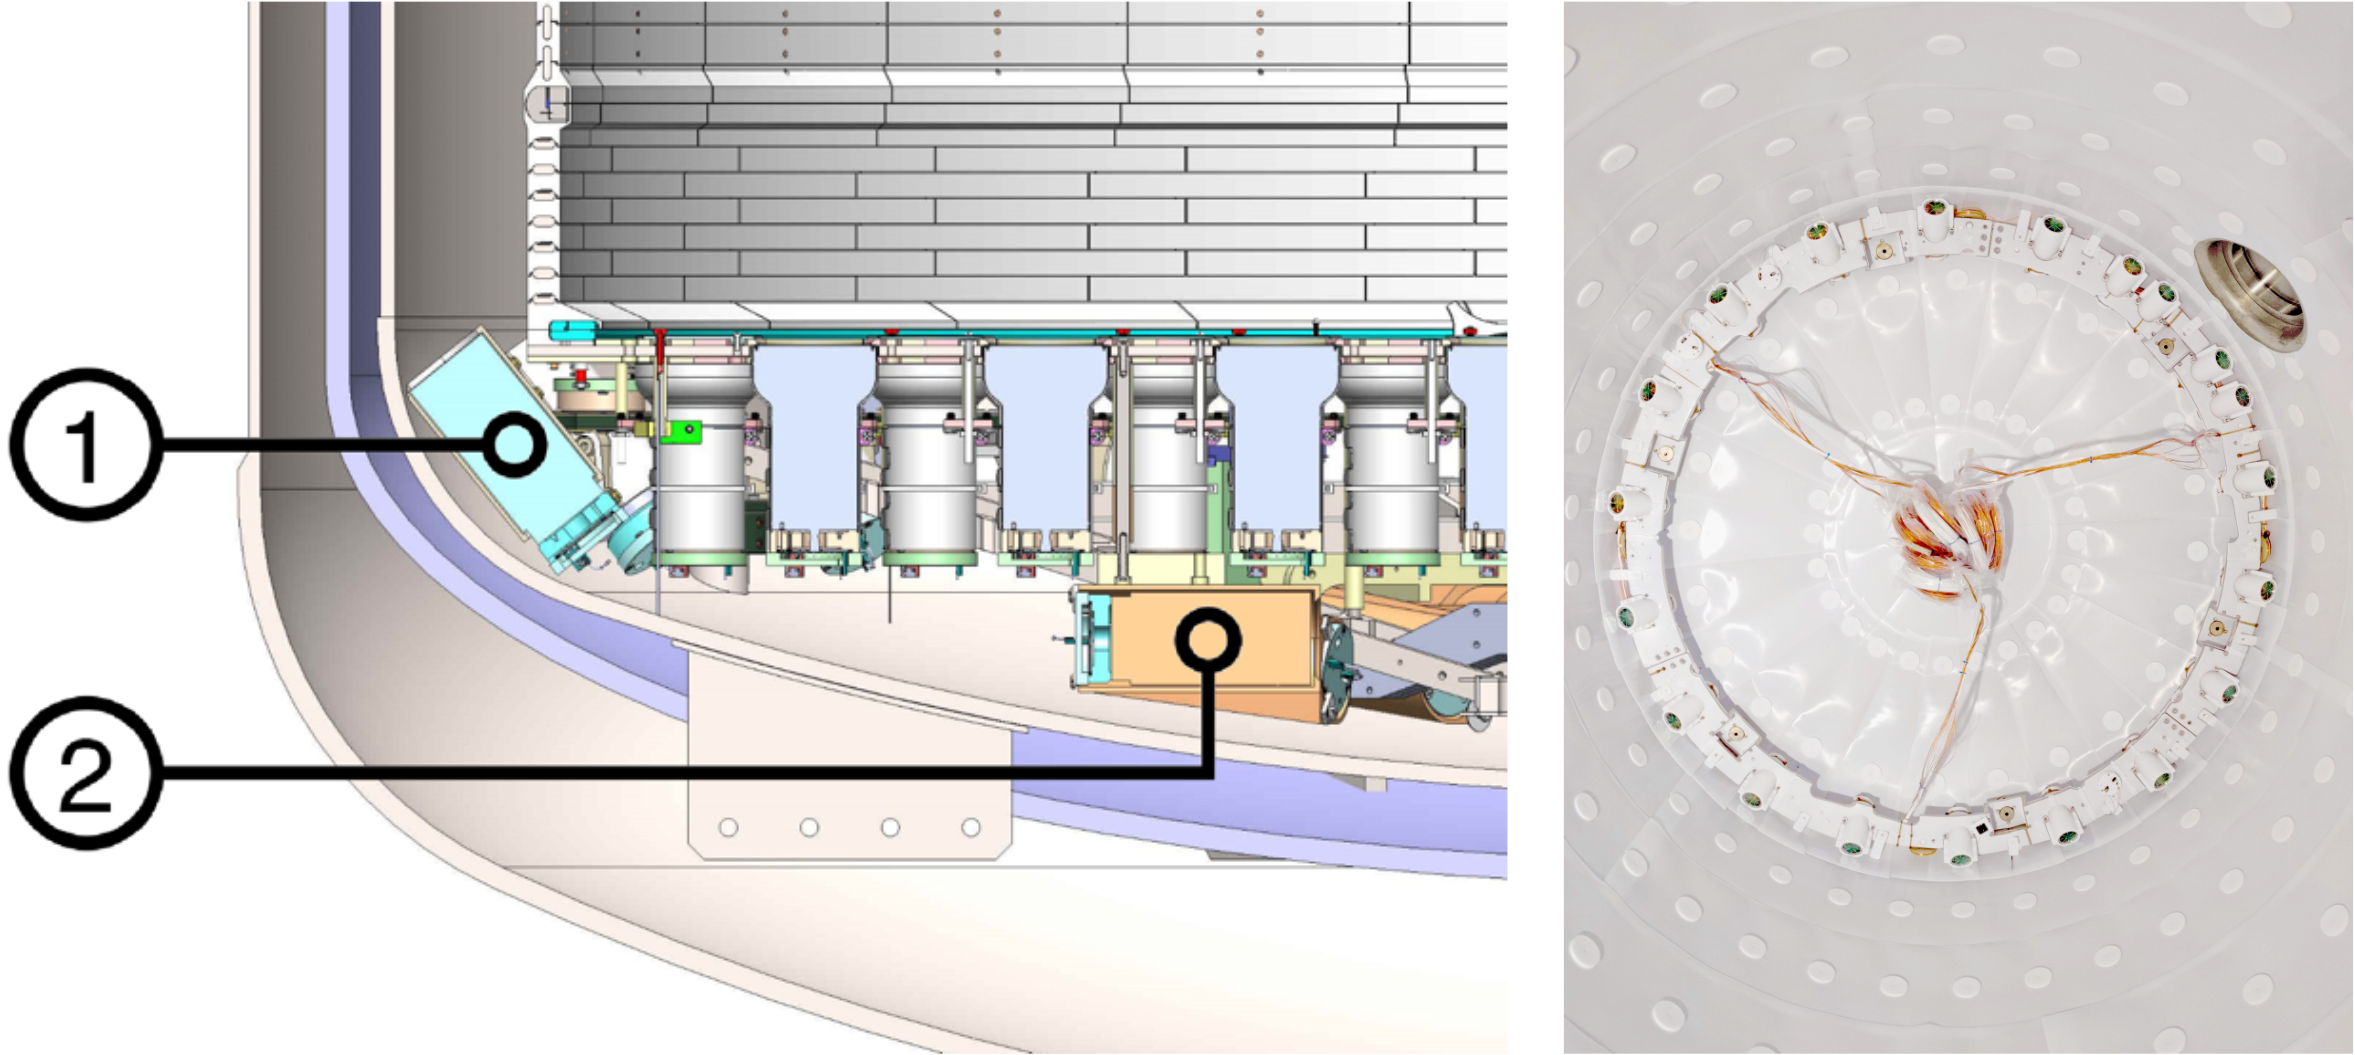
\includegraphics[scale=0.77]{Chapter_2/Figures/Skin_detector.png}
        \caption[CAD diagram (left) showing the TPC below the cathode and a photograph (right), showing the PTFE panelling and the bottom skin PMT array.]%
        {Left: CAD section of the TPC below the cathode showing the location of the 2” bottom side skin (1) and lower dome (2) PMTs. Right: Photograph showing the inner ICV with PTFE panelling on the walls and the lower side skin PMT structure at the bottom of the vessel \cite{Akerib:2019fml}.}
        \label{fig:skin_detector_diagram}
    \end{figure}
}
%

The active volume of the TPC is monitored by two arrays of PMTs. A total of 494 PMTs are divided between the top array with 253 PMTs, and the bottom array with 241 PMTs, respectively. The 3-inch PMTs (model No. R11410-22) were manufactured by Hamamatsu for operation in cold liquid xenon. Furthermore, they were optimised for the detection of VUV luminescence, with an average quantum efficiency of 30.9\% while operating in liquid xenon temperatures, and for low-radioactivity, an excellent single photo-electron (SPE) resolution, and low dark noise. At an operating voltage of 1500 V and 12 dynode stages, a nominal gain of $3.5 \times 10^{6}$ is expected at the end of the signal cable. The PMTs are arranged in close-packed hexagonal patterns to maximise the photocathode coverage and position reconstruction of the S2 signal for interactions near the TPC wall. The array structures are made from low-background titanium sourced as part of the R\&D efforts for LZ \cite{LZ_titanium_selection}. The exposed titanium between the PMTs are covered by interlocking PTFE pieces to maximise VUV reflectance. 

The skin region, sitting outside of the TPC is an important component of the xenon detector. The primary purpose of this region is to serve as a dielectric insulation between the TPC and the ICV. In addition to this, this region is also instrumented with VUV sensitive PMTs to serve as a scintillation-only veto detector, highly effective for \grays{}. The skin veto is composed of two regions: the outer layer of xenon outside of the TPC known as the skin, and the region below the TPC, known as the dome. The skin is monitored by three sets of Hamamatsu PMTs. First of these are a ring of 93 1-inch PMTs (model No. R8520) located at the top of the TPC looking down into the skin, and a further 20 2-inch PMTs (model No. R8778) located at the bottom of the TPC looking up and 18 2-inch PMTs mounted right below the TPC looking into the dome. A schematic of this region is shown in figure \ref{fig:skin_detector_diagram}.


\subsection{Cryogenics \& Xenon Handling}
\label{subsec:crypo_xenon}}

The LZ cryogenic system is designed to contain $\sim$10 tonnes of LXe at 175 K. The xenon detector and majority of the LXe payload is held inside the ICV, 
and vacuum coated with the outer cryostat vessel (OCV). The OCV is supported at the bottom by three legs and the ICV is suspended from the top head of the OCV with a mechanism enabling its levelling from above. The cryostat vessels are fabricated from commercially available pure grade-1 titanium, chosen after an extensive screening campaign to identify the most radio-pure sample within a series of samples taken from different manufacturers, as detailed in \cite{LZ_titanium_selection}.

The ICV consists of a top head and a tapered bottom vessel, connected via a large flange near the top. Its tapered shape is to reduce the electric field near the cathode. The top and the bottom heads of the ICV contain ports for cabling and heat exchanger conduits, with a larger port sitting on the front of the vessel for the high voltage (HV) conduit connection. Whilst the size of the ICV is constrained by the Yates shaft, the OCV is constructed of three segments to overcome this restriction. Similarly, the OCV contains a HV port that aligns with the HV port of the ICV. Furthermore, the OCV also has a port opening to accommodate for the deployment of low energy neutrons that's crucial for calibration.

%
\begin{figure}[b!]
    \centering
    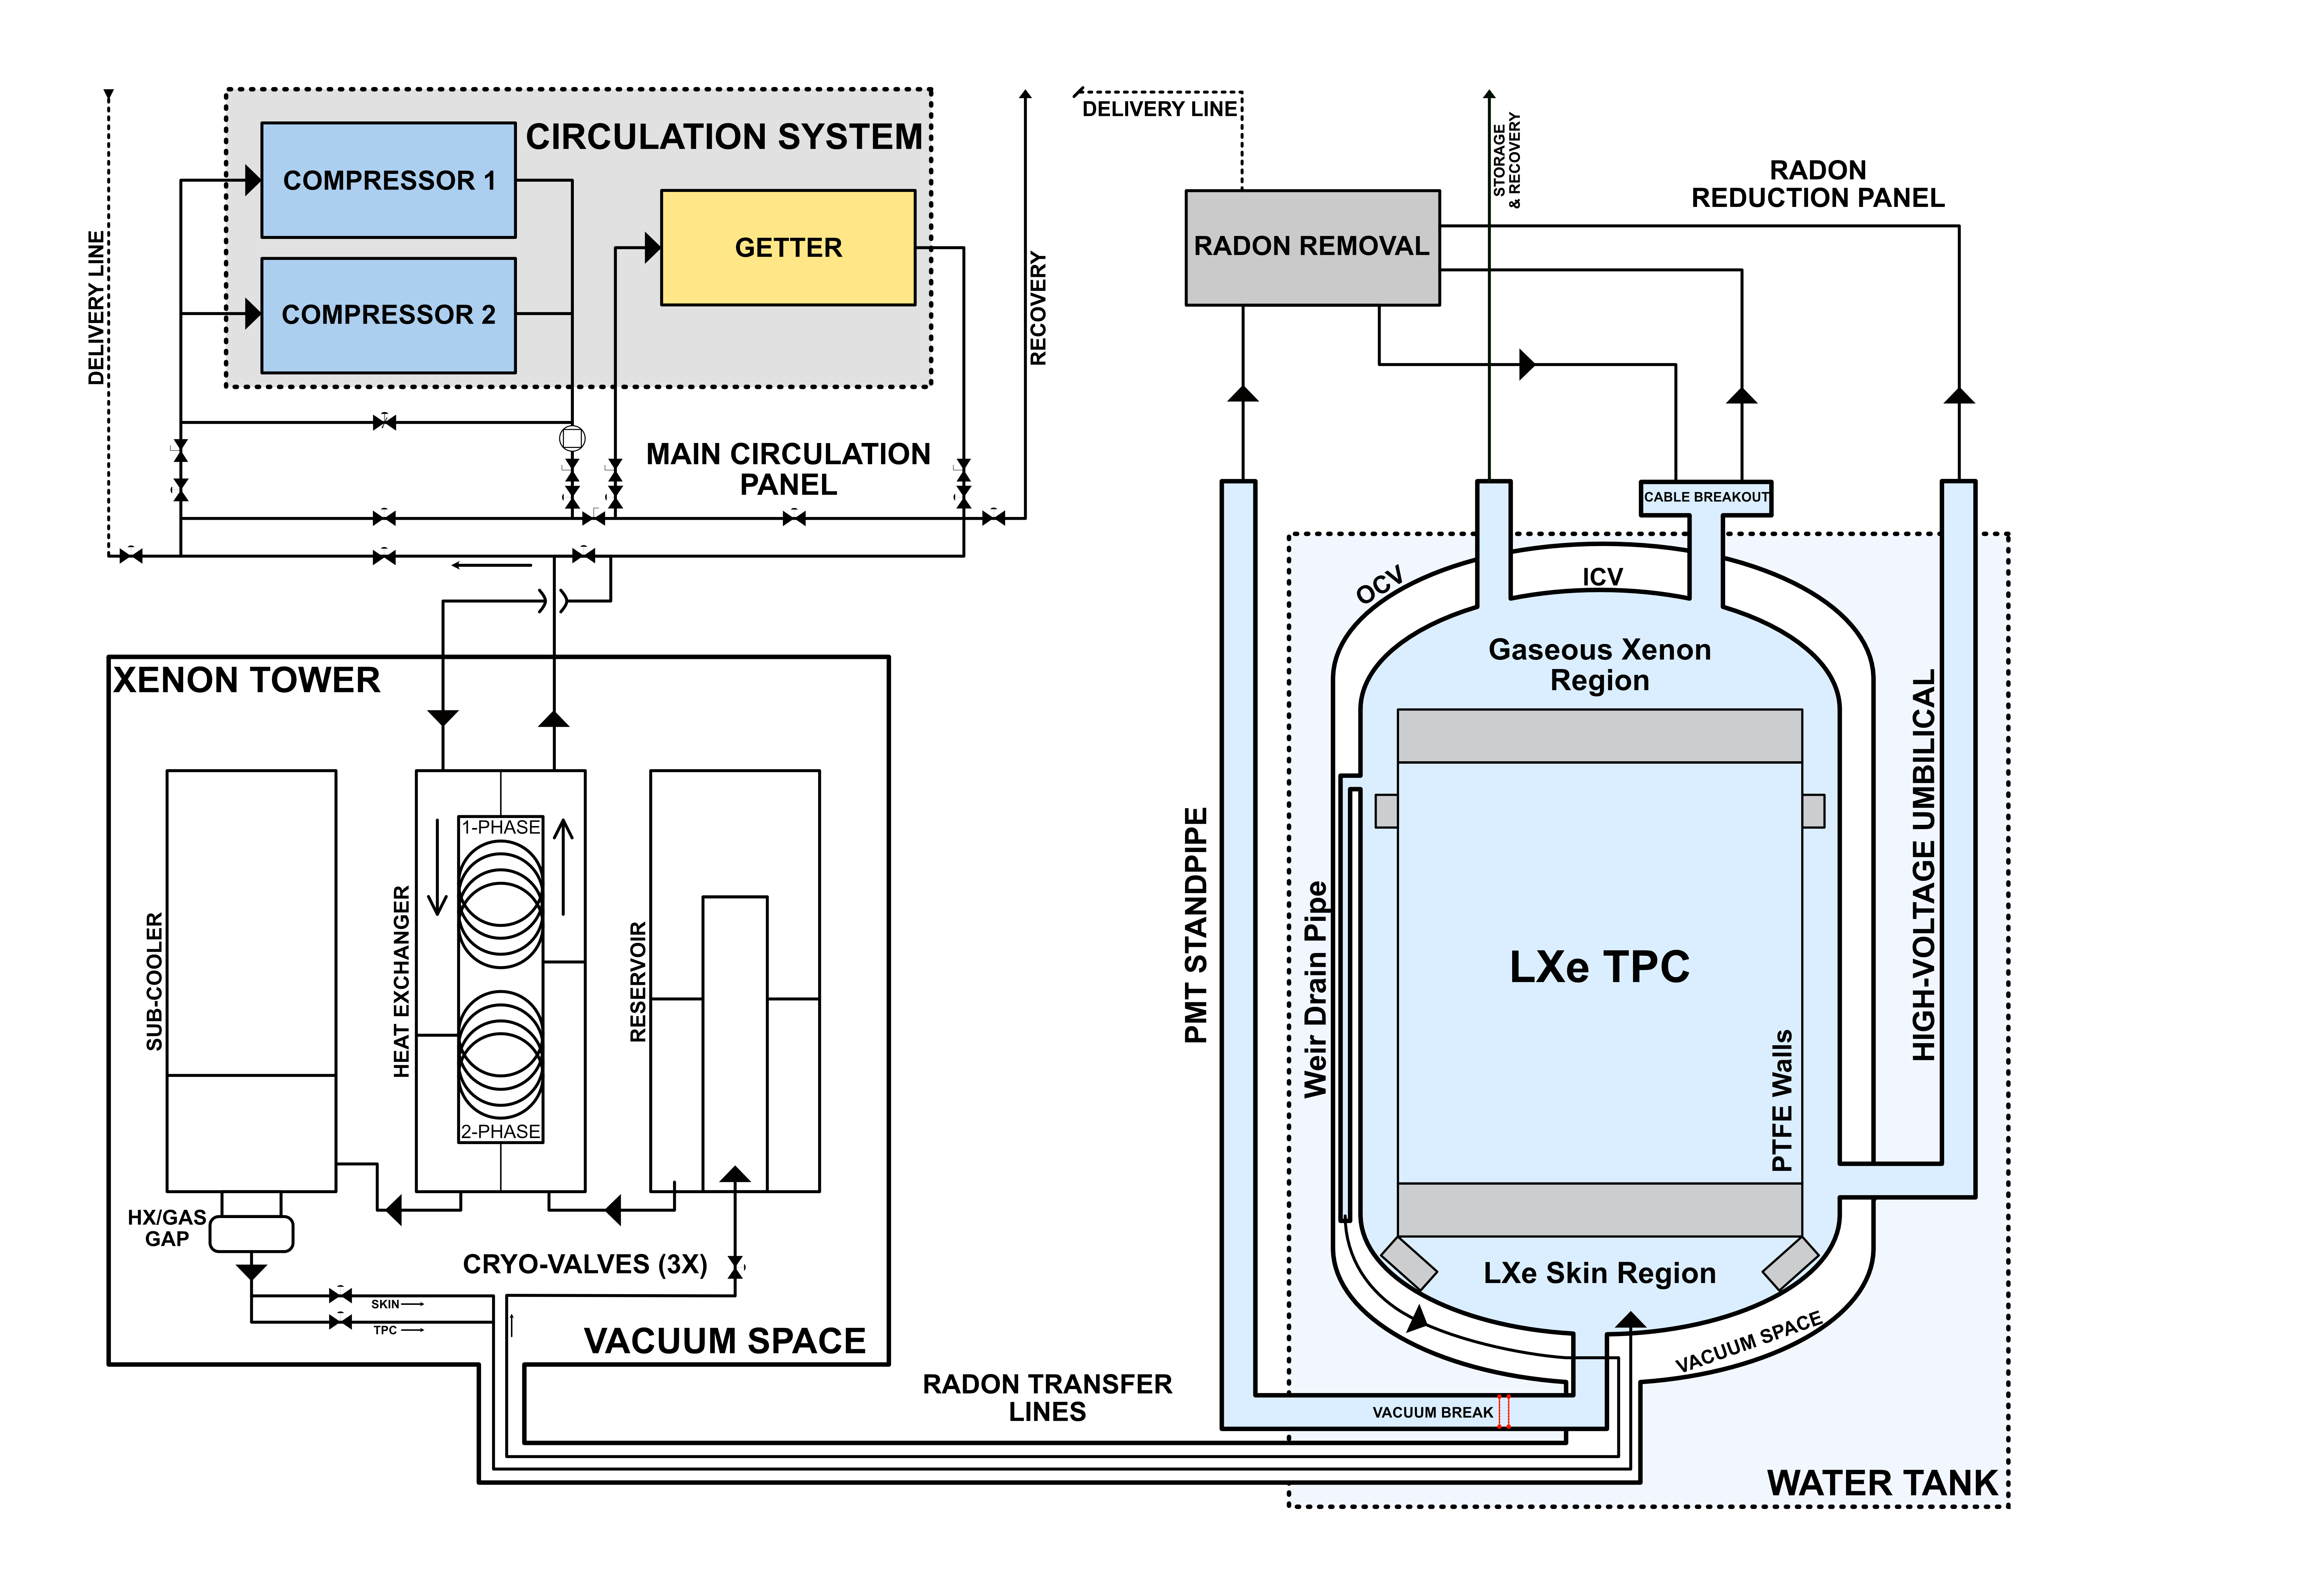
\includegraphics[scale=0.30]{Chapter_2/Figures/LZ_Xenon_Circulation.png}
    \caption[Schematics of the LZ circulation system, detailing TPC, the xenon tower and the compressor systems.]%
    {A simplified overview of the LZ circulation system. Majority of the xenon is held within the TPC, mostly in the liquid phase, with the gaseous region starting just above the weir drain opening. The LXe spills into the weir drain and through the xenon tower, which serves to heat the LXe using a two phase heat exchanger. The gaseous xenon is pumped through a hot zirconium getter, and returned to the detector after condensing. A radon removal system treats Xe gas in the cable conduits and breakout feed-throughs before sending it to the compressor inlet.}
    \label{fig:circulation_diagram}
\end{figure}
%

An overview of the cryogenic and xenon handling systems are shown in the schematic in figure \ref{fig:circulation_diagram}. The temperature inside of the ICV is maintained by a set of closed-loop thermosyphon heat pipes with nitrogen as the process fluid. In operation, the liquid inside of the TPC is drained through the weir pipes, flowing into the xenon tower, which is a cryogenic system sitting outside of the water tank. The tower consists of four vessels: the reservoir vessel, the two-phase heat exchanger (HEX), the subcooler vessel, and the subcooler HEX. The tower acts as a system to convert xenon from either a liquid-to-gas phase or a gas-to-liquid phase. The circulation is established by the use of two all-metal diaphragm gas compressors (model No. A2-5/15) from Fluitron, circulating the gas through a hot zirconium getter at a design flow rate of 500 standard liters per minute (SLPM), taking 2.4 days to purify the full 10 tonne Xe inventory in a single pass. After the removal of electronegative species and calibration sources such as tritium or \COF{}, the xenon is pumped through the cryogenic tower and back into the TPC and the skin region.


\subsection{Outer Detector}
\label{subsec:od}}


The outer detector (OD) system consists of a set of 10 segmented acrylic tanks surrounding the ICV, as highlighted in figure \ref{fig:od_tanks}. The segments are filled with a total of 17.3 tonnes of liquid scintillator. The scintillation medium consists of a linear alkylbenzene (LAB) solvent doped at 0.1\% by mass with gadolinium \cite{YEH2007329}. The primary purpose of the scintillation system is to veto neutrons and \grays{} originating from radioactive impurities in material immediately adjacent to the TPC. The OD is designed to optimise the capture and tagging of neutrons within a time window that allows the signals to be correlated with the NR in the TPC. The secondary purpose of the system is to serve as an additional detector in constructing more accurate background rates for both neutrons and \grays{}. 
%
\begin{figure}[b!]
    \centering
    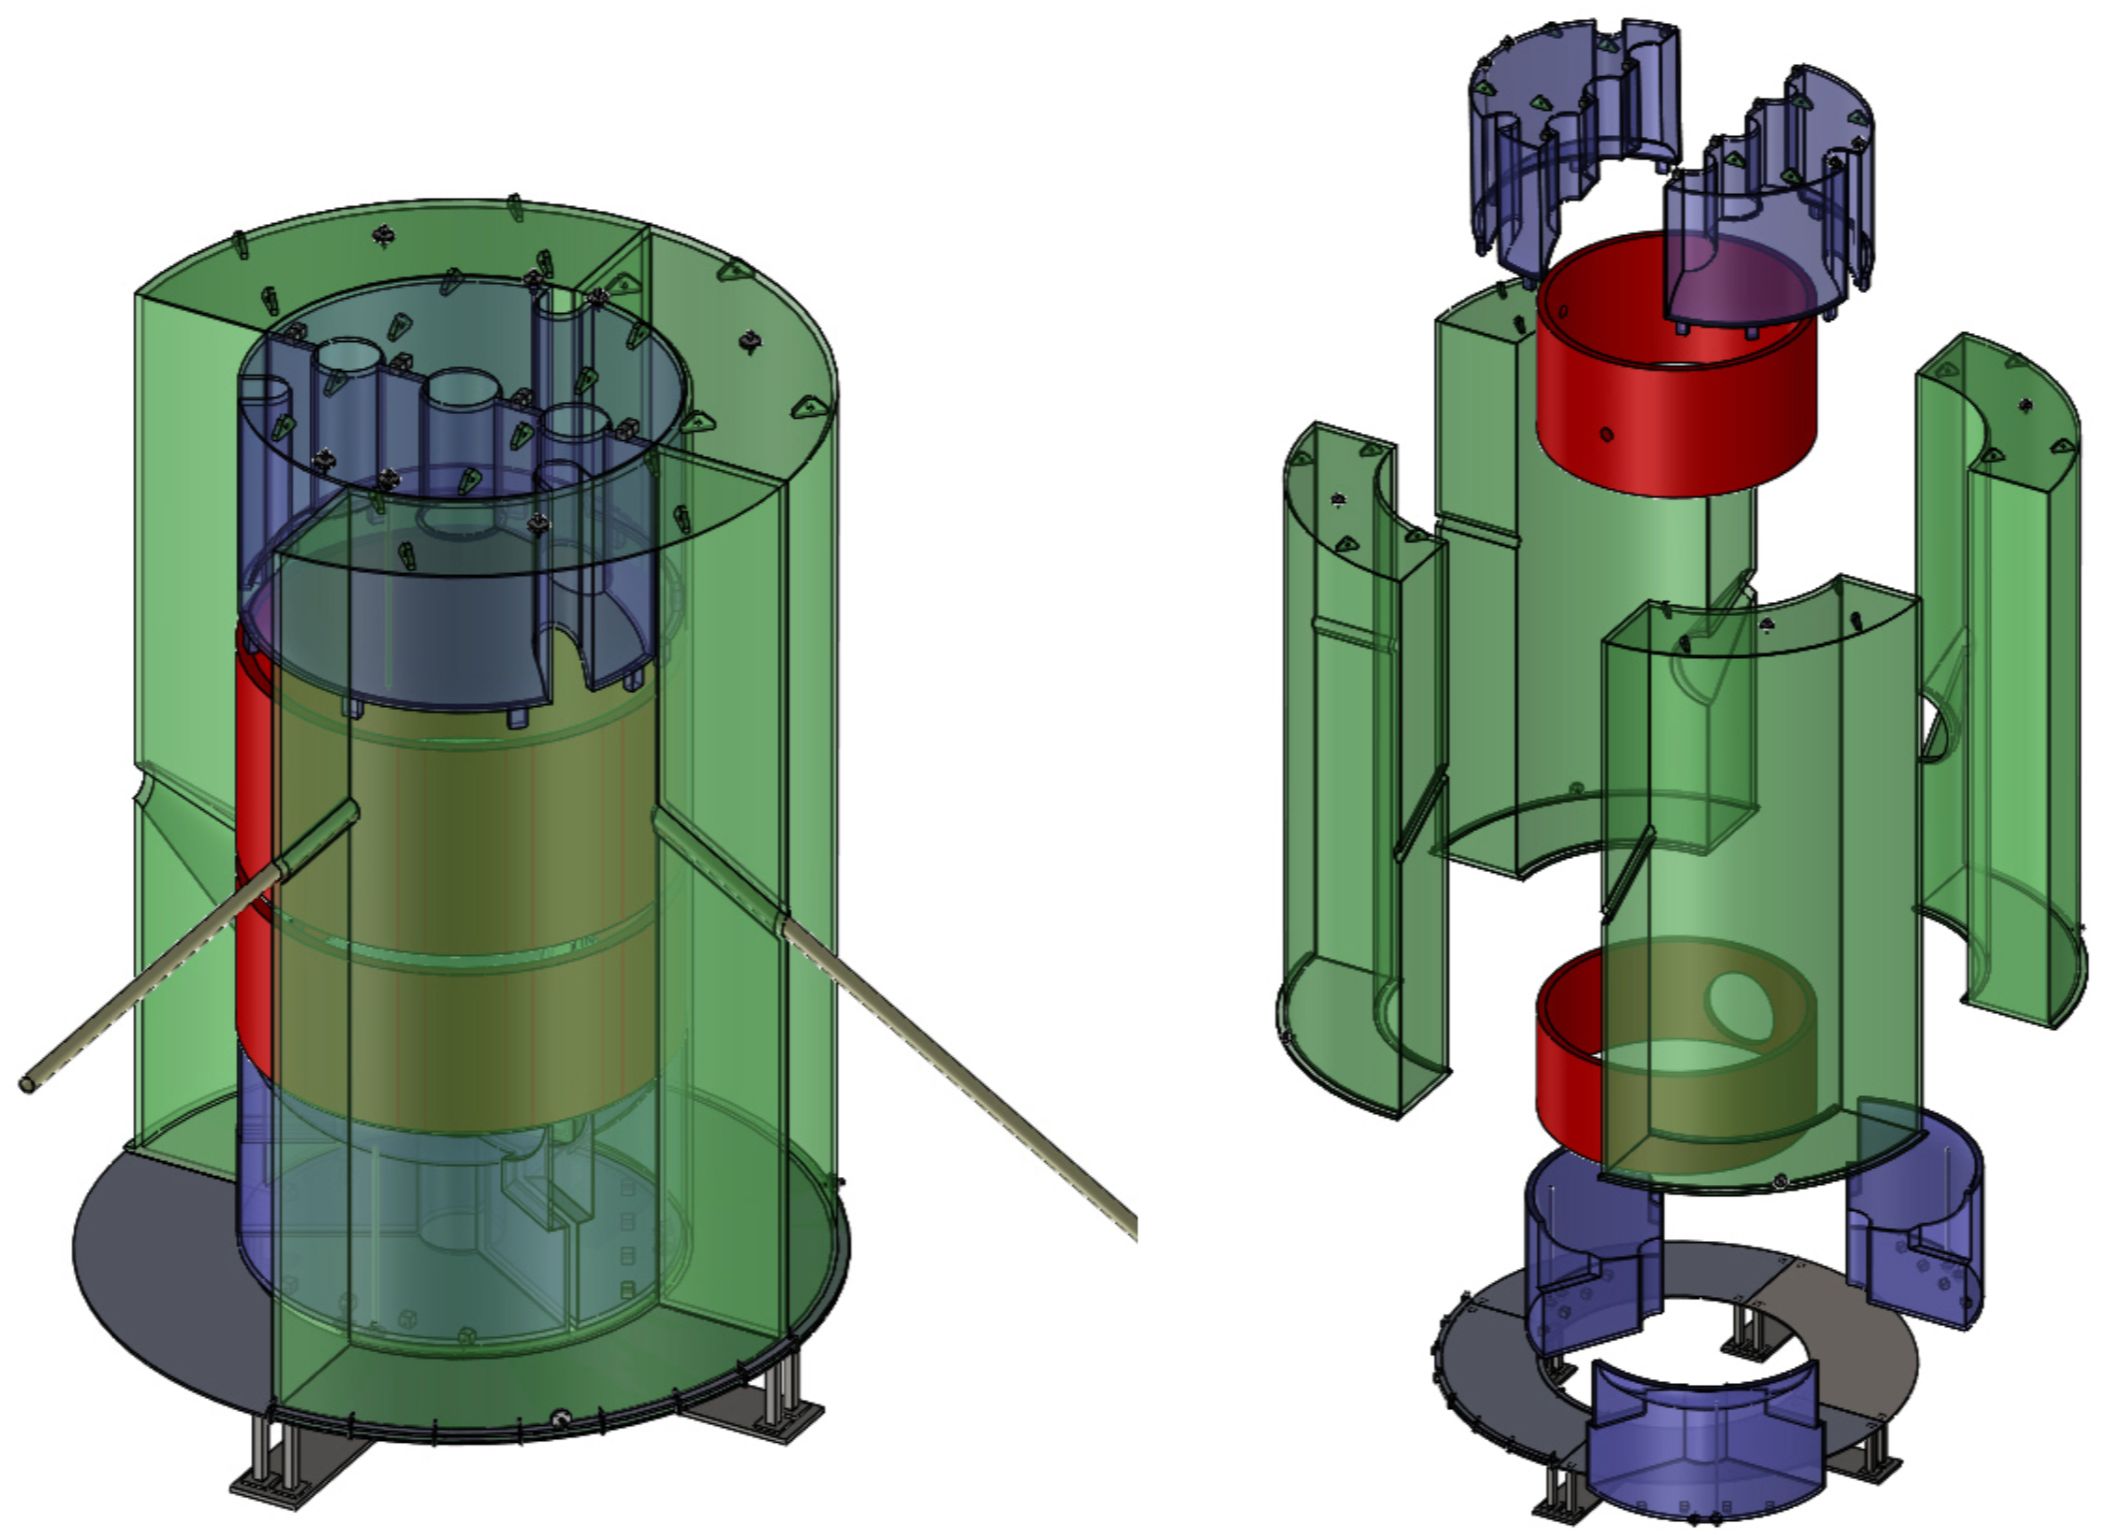
\includegraphics[scale=0.60]{Chapter_2/Figures/LZ_Outer_Detector.png}
    \caption[Schematic diagram of the liquid scintillator acrylic tanks.]%
    {Schematic diagram of the liquid scintillator acrylic tanks. The four green tanks will cover sides, while the blue will cover above and below the OD. Displacer cylinders are shown in red \cite{lz_tdr}.}
    \label{fig:od_tanks}
\end{figure}
%

Most neutrons ($\sim90\%$) are detected predominantly through a neutron capture process with the \gdoFf{} and \gdoFs{} isotopes. Upon capture, multiple \grays{} emitted, totaling 7.9 MeV (\gdoFf) or 8.5 MeV (\gdoFs). The remaining neutrons ($\sim10\%$) are captured on hydrogen, emitting a single 2.2 MeV gamma. The emitted gammas induce scintillation within the GdLS, which are collected by 120 8-inch PMTs arranged in a cylindrical array of 20 ladders that sit on support structures inside of the water tank. The light collection efficiency is further optimised by the use of Tyvek curtain that coat above, below and behind the PMT structure, and a layer surround the cryostat.


\subsection{Calibrations}
\label{subsec:calibrations}

The calibration campaign developed for LZ is a multi-purpose effort to understand accurately and precisely the response of instruments, different detection regions and the underlying xenon response for both ER and NR interactions at varying energy scales. To achieve this, LZ will utilise on internal and external calibration sources, using a range of radioactive nuclide sources. A list of these sources with key highlights are summarised and presented in table \ref{tab:calibration_sources}.

The deployment of internal calibration sources is necessary due to the self-shielding properties of LXe. To overcome this, known amounts of specific isotopes are injected into the circulation system, from which a uniform mixing with LXe in the active region can be achieved. The baseline set of internal sources include short-lived isotopes such as \KrETm{}, \XeOTOm{} and \RnTTZ{} that are stored in the form of their parent nuclide that can be handled and stored in a compact solid form. Additionally, long-lived sources such as \HT{} and \COF{} can be stored as pressurised gas with purified Xe serving as the carrier. The removal of long-lived isotopes is critical and hence their form of deployment must be in a chemical form that can be effectively removed by the getter. Both long-lived and short-lived gaseous sources require precise dose control on the injected activity, accomplished via a gas handling system dedicated to injection control.

The external sources are predominantly used to calibrate nuclear recoil response and are achieved via two distinct methods. The first of these lower sources into the vacuum region between the ICV and the OCV with a deployment system which raises and lowers the source through three conduits with a position accuracy of $\pm5 \; \MathText{mm}$. A selection of photoneutron ($\gamma, n$) sources, as listed in table \ref{tab:calibration_sources}, are planned to calibrate the nuclear recoil energy range from below 1 keV up to about 4.6 keV. This energy region is of particular interest as \BE{} solar neutrino coherent scattering falls within this window. A second method to calibrate higher energy NR response is by using a deuterium-deuterium (DD) neutron generator that produces up to $10^{8}$ neutrons per second. The setup will sit outside of the water tank delivering neutrons through the outer detector via a dedicated neutron conduits. This source has already been used by LUX to obtain a precise, in-situ calibration of the low-energy nuclear recoil response \cite{lux_dd}.

\begin{table}[h]
\centering
\caption
[Overview of the radioactive nuclide sources planned for LZ calibration, highlighting the type of interaction, energy deposition range, half-life of the isotopes and their intended purpose.]
{Overview of the radioactive nuclide sources planned for LZ calibration, highlighting the type of interaction, energy deposition range, half-life of the isotopes and their intended purpose. The partitioned sections represent different deployment techniques. 1$^{st}$: Internal gaseous sources. 2$^{nd}$: Sealed sources lowered down small-diameter conduits to cryostat side vacuum, 3$^{rd}$: \gammaN{} sources that are deployed as indicated in (2), but require dense shielding. 4$^{th}$: DD generator sources, in which neutrons travel through conduits from the generator.}
\label{tab:calibration_sources}
\vspace{1mm}
\renewcommand{\arraystretch}{1.2}
    \begin{tabularx}{1.0\linewidth}{@{\extracolsep{\fill}}lllll}
    \toprule
    
    \textbf{Isotope} & %1
    \textbf{Type} & %2
    \textbf{Energy [keV]} & %3
    \textbf{$\tau_{1/2}$} & %4
    \textbf{Purpose} & %5
    \hline
    \hline
    
    \HT{}	 & \beta{}       & 18.6 endpoint    & 12.5 y            & ER band \\ 
    \COF{}	 & \beta{}       & 156 endpoint     & 5730 y            & ER band \\ 
    \KrETm	 & \gamma{}      & 9.4, 32.1        & 1.83 h            & TPC ($x,y,z$) \\ 
    \XeOTOm	 & \gamma{}      & 164              & 11.8 d            & TPC ($x,y,z$), Xe skin \\ 
    \RnTTZ{} & \alpha{}, \beta{},  \gamma{} & various   & 10.6 h    & Xe skin \\ 
    
    \hline
    
    \NaTT{}	 & \gamma{}       & 511, 1275       & 2.61 y      & TPC and OD sync \\ 
    \MnFF{}	 & \gamma{}       & 835             & 312 d       & High-energy ER response \\ 
    \CoFS{}	 & \gamma{}       & 122             & 0.74 y      & Xe skin \\ 
    \CoSZ{}	 & \gamma{}       & 1173 , 1333     & 5.27 y      & High-energy ER response \\ 
    \BaOTT{} & \gamma{}       & 356             & 10.5 y      & ER response \\ 
    \ThTTE{} & \gamma{}       & 2615            & 1.91 y      & High-energy ER response \\ 
    \AmLi{}	 & \alphaN{}      & 1500 endpoint   & 432 y       & NR band \\ 
    \AmBe{}	 & \alphaN{}      & 11,000 endpoint & 432 y       & NR band \\ 
    \CfTFT{} & \neutron       & Watt spectrum   & 2.65 y      & NR efficiency \\ 
    
    \hline
    
    \YBe{}	    & \gammaN{}     & 152       & 107 d     & NR response \\ 
    \SbBe{}	    & \gammaN{}     & 22.5      & 60.2 d    & NR response \\ 
    \BiBeTZF{}	& \gammaN{}     & 88.5      & 15.3 d    & NR response \\ 
    \BiBeTZS{}	& \gammaN{}     & 47        & 6.24 d    & NR response \\ 
    
    \hline
    
    \DD{}	& \neutron{}        & 272 \xrightarrow{} 400        & ---     & NR light and charge yields \\ 
    \DD{}	& \neutron{}        & 2450                          & ---     & NR light and charge yields \\
    
    \bottomrule
    \end{tabularx}
\end{table}